% This is the Reed College LaTeX thesis template. Most of the work
% for the document class was done by Sam Noble (SN), as well as this
% template. Later comments etc. by Ben Salzberg (BTS). Additional
% restructuring and APA support by Jess Youngberg (JY).
% Your comments and suggestions are more than welcome; please email
% them to cus@reed.edu
%
% See https://www.reed.edu/cis/help/LaTeX/index.html for help. There are a
% great bunch of help pages there, with notes on
% getting started, bibtex, etc. Go there and read it if you're not
% already familiar with LaTeX.
%
% Any line that starts with a percent symbol is a comment.
% They won't show up in the document, and are useful for notes
% to yourself and explaining commands.
% Commenting also removes a line from the document;
% very handy for troubleshooting problems. -BTS

% As far as I know, this follows the requirements laid out in
% the 2002-2003 Senior Handbook. Ask a librarian to check the
% document before binding. -SN

%%
%% Preamble
%%
% \documentclass{<something>} must begin each LaTeX document
\documentclass[12pt,twoside]{reedthesis}
% Packages are extensions to the basic LaTeX functions. Whatever you
% want to typeset, there is probably a package out there for it.
% Chemistry (chemtex), screenplays, you name it.
% Check out CTAN to see: https://www.ctan.org/
%%
\usepackage{graphicx,latexsym}
\usepackage{amsmath}
\usepackage{amssymb,amsthm}
\usepackage{longtable,booktabs,setspace}
\usepackage{chemarr} %% Useful for one reaction arrow, useless if you're not a chem major
\usepackage[hyphens]{url}
% Added by CII
\usepackage{hyperref}
\usepackage{lmodern}
\usepackage{float}
\floatplacement{figure}{H}
% Thanks, @Xyv
\usepackage{calc}
% End of CII addition
\usepackage{rotating}

% Next line commented out by CII
%%% \usepackage{natbib}
% Comment out the natbib line above and uncomment the following two lines to use the new
% biblatex-chicago style, for Chicago A. Also make some changes at the end where the
% bibliography is included.
%\usepackage{biblatex-chicago}
%\bibliography{thesis}
% \ifxetex
%   \usepackage{polyglossia}
%   \setmainlanguage{spanish}
%   % Tabla en lugar de cuadro
%   \gappto\captionsspanish{\renewcommand{\tablename}{Tabla}
%           \renewcommand{\listtablename}{Índice de tablas}}
% \else
%   \usepackage[spanish,es-tabla]{babel}
% \fi

% Added by CII (Thanks, Hadley!)
% Use ref for internal links
\renewcommand{\hyperref}[2][???]{\autoref{#1}}
\def\chapterautorefname{Chapter}
\def\sectionautorefname{Section}
\def\subsectionautorefname{Subsection}
% End of CII addition

% Added by CII
\usepackage{caption}
\captionsetup{width=5in}
% End of CII addition

% \usepackage{times} % other fonts are available like times, bookman, charter, palatino

% Syntax highlighting #22
  \usepackage{color}
  \usepackage{fancyvrb}
  \newcommand{\VerbBar}{|}
  \newcommand{\VERB}{\Verb[commandchars=\\\{\}]}
  \DefineVerbatimEnvironment{Highlighting}{Verbatim}{commandchars=\\\{\}}
  % Add ',fontsize=\small' for more characters per line
  \usepackage{framed}
  \definecolor{shadecolor}{RGB}{248,248,248}
  \newenvironment{Shaded}{\begin{snugshade}}{\end{snugshade}}
  \newcommand{\AlertTok}[1]{\textcolor[rgb]{0.94,0.16,0.16}{#1}}
  \newcommand{\AnnotationTok}[1]{\textcolor[rgb]{0.56,0.35,0.01}{\textbf{\textit{#1}}}}
  \newcommand{\AttributeTok}[1]{\textcolor[rgb]{0.77,0.63,0.00}{#1}}
  \newcommand{\BaseNTok}[1]{\textcolor[rgb]{0.00,0.00,0.81}{#1}}
  \newcommand{\BuiltInTok}[1]{#1}
  \newcommand{\CharTok}[1]{\textcolor[rgb]{0.31,0.60,0.02}{#1}}
  \newcommand{\CommentTok}[1]{\textcolor[rgb]{0.56,0.35,0.01}{\textit{#1}}}
  \newcommand{\CommentVarTok}[1]{\textcolor[rgb]{0.56,0.35,0.01}{\textbf{\textit{#1}}}}
  \newcommand{\ConstantTok}[1]{\textcolor[rgb]{0.00,0.00,0.00}{#1}}
  \newcommand{\ControlFlowTok}[1]{\textcolor[rgb]{0.13,0.29,0.53}{\textbf{#1}}}
  \newcommand{\DataTypeTok}[1]{\textcolor[rgb]{0.13,0.29,0.53}{#1}}
  \newcommand{\DecValTok}[1]{\textcolor[rgb]{0.00,0.00,0.81}{#1}}
  \newcommand{\DocumentationTok}[1]{\textcolor[rgb]{0.56,0.35,0.01}{\textbf{\textit{#1}}}}
  \newcommand{\ErrorTok}[1]{\textcolor[rgb]{0.64,0.00,0.00}{\textbf{#1}}}
  \newcommand{\ExtensionTok}[1]{#1}
  \newcommand{\FloatTok}[1]{\textcolor[rgb]{0.00,0.00,0.81}{#1}}
  \newcommand{\FunctionTok}[1]{\textcolor[rgb]{0.00,0.00,0.00}{#1}}
  \newcommand{\ImportTok}[1]{#1}
  \newcommand{\InformationTok}[1]{\textcolor[rgb]{0.56,0.35,0.01}{\textbf{\textit{#1}}}}
  \newcommand{\KeywordTok}[1]{\textcolor[rgb]{0.13,0.29,0.53}{\textbf{#1}}}
  \newcommand{\NormalTok}[1]{#1}
  \newcommand{\OperatorTok}[1]{\textcolor[rgb]{0.81,0.36,0.00}{\textbf{#1}}}
  \newcommand{\OtherTok}[1]{\textcolor[rgb]{0.56,0.35,0.01}{#1}}
  \newcommand{\PreprocessorTok}[1]{\textcolor[rgb]{0.56,0.35,0.01}{\textit{#1}}}
  \newcommand{\RegionMarkerTok}[1]{#1}
  \newcommand{\SpecialCharTok}[1]{\textcolor[rgb]{0.00,0.00,0.00}{#1}}
  \newcommand{\SpecialStringTok}[1]{\textcolor[rgb]{0.31,0.60,0.02}{#1}}
  \newcommand{\StringTok}[1]{\textcolor[rgb]{0.31,0.60,0.02}{#1}}
  \newcommand{\VariableTok}[1]{\textcolor[rgb]{0.00,0.00,0.00}{#1}}
  \newcommand{\VerbatimStringTok}[1]{\textcolor[rgb]{0.31,0.60,0.02}{#1}}
  \newcommand{\WarningTok}[1]{\textcolor[rgb]{0.56,0.35,0.01}{\textbf{\textit{#1}}}}

% To pass between YAML and LaTeX the dollar signs are added by CII
\title{Utilización de datos satelitales para la evaluación y mejora de los pronósticos numéricos en alta resolución a muy corto plazo}
\author{Paola Corrales}
% The month and year that you submit your FINAL draft TO THE LIBRARY (May or December)
\date{Algún momento de marzo 2023?}
\division{Facultad de Ciencias Exactas y Naturales}
\advisor{Victoria Galligani}
\institution{Universidad de Buenos Aires}
\degree{Tesis presentada para optar al título de Doctor de la Universidad de Buenos Aires en el área de Ciencias de la Atmósfera y los Oceanos}
%If you have two advisors for some reason, you can use the following
% Uncommented out by CII
\altadvisor{Juan Ruiz}
% End of CII addition

%%% Remember to use the correct department!
\department{Departamento de Ciencias de la Atmósfera y los Oceanos}
% if you're writing a thesis in an interdisciplinary major,
% uncomment the line below and change the text as appropriate.
% check the Senior Handbook if unsure.
%\thedivisionof{The Established Interdisciplinary Committee for}
% if you want the approval page to say "Approved for the Committee",
% uncomment the next line
%\approvedforthe{Committee}

% Added by CII
%%% Copied from knitr
%% maxwidth is the original width if it's less than linewidth
%% otherwise use linewidth (to make sure the graphics do not exceed the margin)
\makeatletter
\def\maxwidth{ %
  \ifdim\Gin@nat@width>\linewidth
    \linewidth
  \else
    \Gin@nat@width
  \fi
}
\makeatother

% From {rticles}

\renewcommand{\contentsname}{Table of Contents}
% End of CII addition

\setlength{\parskip}{0pt}

% Added by CII

\providecommand{\tightlist}{%
  \setlength{\itemsep}{0pt}\setlength{\parskip}{0pt}}

\Acknowledgements{
I want to thank a few people.
}

\Dedication{
You can have a dedication here if you wish.
}

\Preface{
This is an example of a thesis setup to use the reed thesis document class
(for LaTeX) and the R bookdown package, in general.
}

\Abstract{
The preface pretty much says it all.

\par

Second paragraph of abstract starts here.
}

	\usepackage{setspace}\onehalfspacing
	\usepackage{booktabs}
\usepackage{longtable}
\usepackage{array}
\usepackage{multirow}
\usepackage{wrapfig}
\usepackage{float}
\usepackage{colortbl}
\usepackage{pdflscape}
\usepackage{tabu}
\usepackage{threeparttable}
\usepackage{threeparttablex}
\usepackage[normalem]{ulem}
\usepackage{makecell}
\usepackage{xcolor}
% End of CII addition
%%
%% End Preamble
%%
%
\begin{document}

% Everything below added by CII
  \maketitle

\frontmatter % this stuff will be roman-numbered
\pagestyle{empty} % this removes page numbers from the frontmatter
  \begin{acknowledgements}
    I want to thank a few people.
  \end{acknowledgements}
  \begin{preface}
    This is an example of a thesis setup to use the reed thesis document class
    (for LaTeX) and the R bookdown package, in general.
  \end{preface}
  \hypersetup{linkcolor=black}
  \setcounter{secnumdepth}{2}
  \setcounter{tocdepth}{2}
  \tableofcontents

  \listoftables

  \listoffigures
  \begin{abstract}
    The preface pretty much says it all.
    
    \par
    
    Second paragraph of abstract starts here.
  \end{abstract}
  \begin{dedication}
    You can have a dedication here if you wish.
  \end{dedication}
\mainmatter % here the regular arabic numbering starts
\pagestyle{fancyplain} % turns page numbering back on

\hypertarget{introducciuxf3n}{%
\chapter*{Introducción}\label{introducciuxf3n}}
\addcontentsline{toc}{chapter}{Introducción}

\hypertarget{pronostico-de-eventos-severos}{%
\section{Pronostico de eventos severos}\label{pronostico-de-eventos-severos}}

La simulación numérica de la atmósfera, es decir, la integración de las ecuaciones que rigen la evolución del sistema atmósferico es la base para la predicción del tiempo en diversas escalas temporales desde horas a semanas.

La predicción de fenómenos meteorológicos extremos es de particular importancia ya que pueden producir cuantiosas pérdidas humanas y materiales. En Argentina, una gran cantidad de estos fenómenos están asociados a la ocurrencia de convección profunda entre los que se cuentan tornados, ráfagas intensas, precipitaciones extremas en cortos períodos de tiempo, granizo de gran tamaño y actividad eléctrica. Es por tal motivo necesario avanzar en el conocimiento de estos fenómenos y en la capacidad de pronosticar la ocurrencia de los mismos.

El pronostico meteorologico es un problema de condiciones iniciales y de borde. Si se cuenta con condiciones de borde apropiadas, es decir, una correcta representación de las características de la superficie terrestre y el tope de la atmósfera, la generación de pronósticos de calidad dependerá entonces, de la capacidad del modelo para representar los procesos atmosféricos y la exactitud de las condiciones iniciales usadas (Kalnay, 2002).

El pronóstico de los fenómenos severos es a su vez un desafío científico y tecnológico muy complejo debido a la predictibilidad limitada en la mesoescala y debido a la dificultad de conocer o diagnosticar el estado de la atmósfera en escalas espaciales pequeñas y tiempos cortos (por ejemplo de 1 a 10 km y del orden de los minutos).

Uno de los métodos que pueden utilizarse para el pronóstico de fenómenos meteorológicos severos es la utilización de modelos numéricos de la atmósfera que resuelvan explícitamente la convección profunda. Diversos estudios, han comprobado que estos modelos agregan valor al pronóstico a corto plazo y que en muchos casos proveen información sobre el modo de organización de las celdas convectivas y su intensidad (Aksoy et al., 2010; Stensrud et al., 2013). No obstante, la capacidad de los modelos numéricos en anticipar la ubicación y tiempo de ocurrencia de eventos extremos asociados a convección es muy limitada si no se cuenta con una detallada información sobre el estado de la atmósfera en la escala de las tormentas en el momento en el que se inicializan los pronósticos numéricos (Clark et al., 2009).

\hypertarget{asimilaciuxf3n-de-datos-como-posible-soluciuxf3n}{%
\section{Asimilación de datos como posible solución}\label{asimilaciuxf3n-de-datos-como-posible-soluciuxf3n}}

Por otro lado es posible aplicar técnicas de asimilación de datos para generar una mejor estimación de las condiciones iniciales necesarias para integrar un modelo numérico. La asimilación de datos combina de manera optima un pronóstico numérico o campo preliminar en un tiempo t con las observaciones disponibles para ese mismo tiempo, generando un análisis. Esta combinación optima toma en cuenta el error asociado al modelo meteorológico (errores de pronóstico) y el error de las observaciones (que resulta de los errores instrumentales y los errores de representatividad) y su error será menor a los errores originales. Por esta razón el análisis es considerado desde un punto de vista estadistico y bajo ciertas hipotesis, como la \emph{mejor aproximación} disponible del estado real de la atmósfera.


\begin{figure}

{\centering 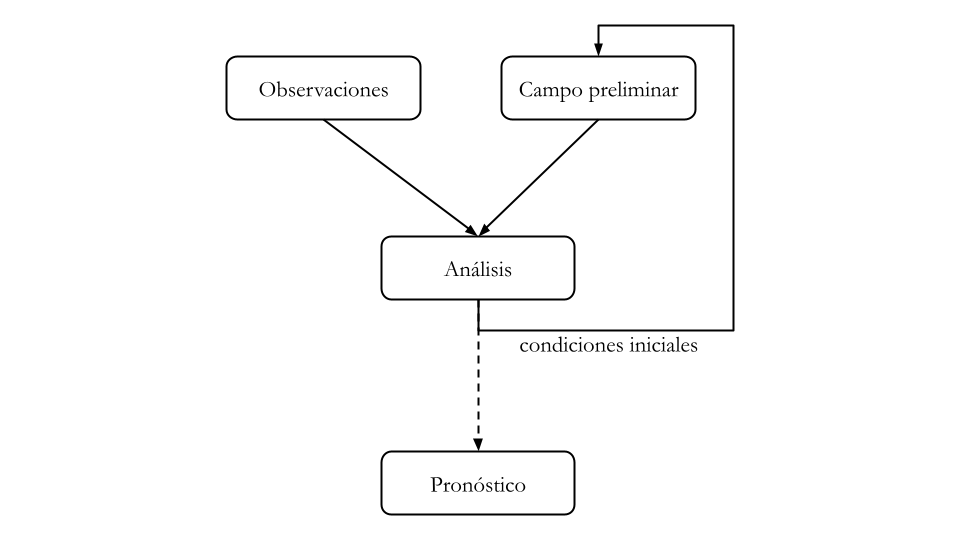
\includegraphics[width=1\linewidth]{/home/paola.corrales/tesis_doctorado/figure/ciclo_asimilacion_teorico} 

}

\caption{Esquema de un ciclo de asimilación típico. El tiempo de las observaciones y el campo preliminar deberá coincidir.}\label{fig:ciclo-asimilacion-teorico}
\end{figure}
Un ciclo de asimilación de datos típico se muestra en la Figure \ref{fig:ciclo-asimilacion-teorico}. En un tiempo dado se comparan las observaciones disponibles con el campo preliminar para ese mismo tiempo, generando así el análisis que se utilizará como condición inicial para un futuro pronóstico o campo preliminar. En el caso de modelos globales, típicamente cada ciclo de asimilación de 6 horas utiliza el campo preliminar previo, es decir el pronóstico a 6 horas inicializado a partir del análisis anterior y las observaciones disponibles para las 6 horas previas o en un periodo similar centrado en la hora del análisis.
Para poder comparar y combinar el campo preliminar con las observaciones, este es interpolado a la ubicación de las observaciones. En determinados casos, por ejemplo cuando se trabaja con observaciones de satélite o radar, será necesario transformar las variables del modelo para obtener las variables observadas. En la siguiente ecuación \(H\) es el operador de las observaciones no lineal que se encarga de las interpolaciones y transformaciones necesarias sobre el campo preliminar \(x_b\).
\begin{equation}
  \mathrm{x_a = x_b + W[y_o - H(x_b )]}
  \label{eq:eq1}
\end{equation}
La diferencia entre las observaciones \(y_o\) y el campo preliminar se denomina innovación. El análisis \(x_a\) se obtiene aplicando las innovaciones al campo preliminar teniendo en cuenta un peso \(W\) que incluye información sobre los errores del pronóstico y de las observaciones.

Existen diferentes metodologías para obtener \(x_a\). Los métodos variacionales, 3D-Var y 4D-Var, definen una función de costo que es proporcial a la distancia entre el análisis y el campo preliminar y el análisis y las obvservaciones simultaneamente. Esta función de costo \(J\) es minimizada para obtener el análisis.
\begin{equation}
  \mathrm{J = \frac{1}{2} {[y_o - H (x_a)]^T R^{-1} [y_o - H (x_a)] + (x_a - x_b )^T B^{-1} (x_a - x_b )}}
  \label{eq:eq2}
\end{equation}
En la ecuación \eqref{eq:eq2}, el primer término corresponde a la distancia entre el campo del análisis y las observaciones, pesado por la covarianza de los errores de las observaciones \(R\). El segundo término a la distancia entre el campo del análisis y el campo preliminar pesado por la covarianza de los errores del pronóstico \(B\). Para el caso más simple, es decir, una variable de modelo y una observación, \(R\) y \(B\) son escalares. Para el caso multidimensional, serán matrices de covarianza de dimension \(n\) (número de observaciones) que deben ser estimadas. Las ecuaciones \eqref{eq:eq1} y \eqref{eq:eq2} son equivalentes si \(H\) es un operador lineal y si se define a W como:
\begin{equation}
  \mathrm{W = BH^T (HBH^T + R^{-1})^{-1}}
  \label{eq:eq3}
\end{equation}
El método 4D-Var extiende el uso del método 3D-Var para incluir la distancia a las observaciones que pueden estar distribuidas temporalmente dentro de la ventana de asimilación en la misma función de peso. Sin embargo minimizar la función de costo requiere desarrollar el modelo tangente lineal y su adjunto, lo que puede ser costoso cuando se trabaja con modelos no lineales. Por esta misma razón, obtener la matriz \(B\) es un problema complejo y en general se la asume constante en el tiempo.

Los métodos secuenciales y en particular el filtro de Kalman extendido, actualizan el análisis a medida que las observaciones están disponibles. Este método tiene además la ventaja de actualizar la matriz \(B\) junto con el análisis. En este caso la matriz \(W\) toma el nombre de \(K\) o ganancia de Kalman que también actualiza en cada ciclo de asimilación \(t_i\).
\begin{equation}
  \mathrm{K_i = B(t_i) H^T (HB(t_i)H^T + R^{-1})^{-1}}
  \label{eq:eq4}
\end{equation}
La estimación de \(B\) utilizando el filtro de Kalman extendido es particularmente costosa en terminos computacionales por lo que que en la práctica se utiliza el filtro de Kalman por ensambles o EnKF. Un ensamble consiste en un conjunto de simulaciones ligeramente diferentes que se resuelven simultaneamente para incluir los posibles estados de la atmósfera y provee información dependiente de la dinámica durante la ventana de asimilación. A partir del ensamble, la matriz \(B\) se estima como:
\begin{equation}
  \mathrm{ B \approx \frac{1}{m-1} \sum_{k=1}^{m}(x_{b}^{k}-\overline{x}_b)(x_{b}^{k}-\overline{x}_b)^T}
  \label{eq:eq5}
\end{equation}
donde \(k \; \epsilon \; [1,m]\) el miembro \emph{k-ésimo} del ensamble. Esta estimación será buena si el ensamble logra capturar los posibles estados futuros o en otras palabras el spread que acompañe los cambios en la incertidumbre de los pronosticos a lo largo de los ciclos de asimilación. Sin embargo, este método no es aplicable a menos que el tamaño del ensamble sea comparable a los grados de libertad de un modelo que resuelve \(10^9\) variables de estado, lo que resulta computacionalmente inviable.

El método Local Ensemble Transform Kalman Filter (LETKF) busca resolver los problemas anteriores resoloviendo las ecuaciones previas en un espacio de dimensión reducida definido por los miembros del ensable. Cómo en el resto de los métodos usando filtro de Kalman, se localiza o restringe el área de influencia de las observaciones a un determinado radio de localización reduciendo el costo computacional necesario. Además, calcula el análisis para cada punto de retícula uno a uno, incorporando todas las observaciones que puedan tener influencia en ese punto al mismo tiempo. De esta manera este método es hasta un orden de magnitud más rápido comparado con otros métodos desarrollados previamente (Whitaker et al., 2008).

Independientemente de la metodología aplicada, el modelo cumple un rol fundamental en la asimilación de datos ya que \emph{transporta} información de regiones donde existe mucha información disponible (por ejemplo, los continentes) a regiones donde las observaciones son escasas (zonas oceánicas) manteniendo los balances físicos que que rigen los procesos atmosféricos.

\hypertarget{resultados-previos-de-asimilaciuxf3n-de-distintas-fuentes-de-observaciones}{%
\section{Resultados previos de asimilación de distintas fuentes de observaciones}\label{resultados-previos-de-asimilaciuxf3n-de-distintas-fuentes-de-observaciones}}

Para que los métodos de asimilación de datos tengan éxito, deben utilizarse redes de observación con suficiente resolución temporal y espacial capaces de captar la variabilidad en las escalas que se quieren resolver, por ejemplo, la mesoescala.

Wheatley and Stensrud (2010) investigó el impacto de la asimilación de datos de presión de superficie en un sistema de asimilación de datos basado en conjuntos de mesoescala, pero encontró un impacto limitado en dos estudios de caso relacionados con sistemas convectivos de mesoescala. Ha and Snyder (2014) demostraron que la asimilación de la temperatura y la temperatura del punto de rocío de las redes de estaciones meteorológicas de superficie de alta resolución mejoraba sistemáticamente la estructura de la capa límite planetaria simulada y mejoraba la previsión de precipitaciones de corto alcance sobre los Estados Unidos. Chang et al. (2017), Bae and Min (2022) y Chen et al. (2016) informaron sobre los efectos beneficiosos de la asimilación de observaciones de estaciones meteorológicas de superficie en un sistema de asimilación de datos de alta resolución utilizando las metodologías de EnKF, 3D-Var y 4D-Var encontrando impactos positivos en el pronóstico de la temperatura y la humedad en la capa límite planetaria y en la localización de los sistemas de precipitación. Sobash and Stensrud (2015) demostró en un sistema de asimilación de datos de mesoescala que el impacto sobre la iniciación de la convección y el pronóstico de la precipitación de corto alcance es positivo si los datos se asimilan con frecuencia (en el orden de minutos, en lugar de en el orden de horas). Maejima et al. (2019) investigaron el impacto de la asimilación con frecuencia de 1 minutos de observaciones sintéticas en un caso de precipitación intensa, encontrando que la asimilación de observaciones de alta frecuencia y espacialmente espacialmente densas conducen a una mejor representación de la circulación de mesoescala aunque el número de observaciones proporcionadas por las estaciones de superficie es mucho menor que el proporcionado por los radares meteorológicos. Gasperoni et al. (2018) realizó un estudio de caso para evaluar el impacto de la asimilación de las observaciones producidas por estaciones meteorológicas privadas que no se incorporan a los análisis operativos globales. Encontró un efecto positivo al asimilar estas observaciones sobre el inicio de la convección húmeda profunda a lo largo de una línea seca. Este resultado es especialmente importante para regiones con pocos datos, como el sur de Sudamérica, donde las redes operativas no son lo suficientemente densas como para captar los detalles de la mesoescala. En ese sentido, Dillon et al. (2021) utilizaron por primera vez observaciones de estaciones meteorológicas automáticas de redes privadas en el sur de Sudamérica, sin embargo, la contribución específica de este tipo de observaciones sobre esta región, no ha sido investigada hasta ahora.

Se ha investigado el impacto de otros tipos de observaciones de resolución espacial y temporal relativamente alta, como observaciones de satélites, en el contexto de la asimilación de datos de mesoescala. Estas observaciones incluyen radianzas y productos derivados como vientos derivados de satélite y perfiles de temperatura y humedad, Wu et al. (2014), Cherubini et al. (2006) y Sawada et al. (2019) observaron un impacto positivo de la asimilación de viento derivado de información satelital de alta frecuencia en un estudio de caso de un ciclón tropical utilizando un sistema de asimilación de datos basado en ensambles. Por otro lado, Gao et al. (2015) observaron un impacto positivo en pronósticos a corto plazo gracias a la asimilación de viento estimado a partir de las observaciones de satélites geoestacionarios sobre Estados Unidos.

\hypertarget{asimilaciuxf3n-de-radianzas-de-satuxe9lites}{%
\subsection{Asimilación de radianzas de satélites}\label{asimilaciuxf3n-de-radianzas-de-satuxe9lites}}

En esta sección se resumirá los alvances en la asimilación de estas observaciones a nivel global y regional.

Los primeros satélites en proveer información meteorológica fueron desarrollados en las décadas de los 60 y 70. Estos estaban ubicados en órbitas polares, es decir, con cierta inclinación respecto del Ecuador, pasando cerca o sobre los polos. Incluian sensores infrarrojos y de microondas para monitorear la temperatura y humedad. Hacia finales de la década de los 70, Estados Unidos, Europa y Japón ya habían lazando los primeros satélites geoestacionarios. Pocos años despues este tipo de observaciones se incorporaban al Sistema de Observación Global (Global Observing System en inglés).

El primer conjunto de satélites compuesto por los sensores High-resolution Infrared Radiation Sounder (HIRS), Microwave Sounding Units (MSU) y Stratospheric Sounder Unit (SSU) o sistema TOVS (por su nombre en inglés, TIROS Operational Vertical Sounder) podían cubrir el globo completo cada 12 hs. Si bien cada uno de estos sensores generaba información complementaria en la tropósfera y baja estratósfera, la resolución horizontal y vertical era limitada. En particular el primer HIRS, un sensor infrarrojo tenía una resolución horizontal de 40 km, mientras que actualmente HIRS4 tiene una resolución horizontal de 10 km. MSU, sensor sensible en las microondas, tenía una resolución de 110 km mientras que el sensor que lo reemplazó, Advanced Microwave Sounding Unit-A (AMSU-A) cuenta con una resoluciónde 50 km. En la vertical, el ancho la función de peso de los distintos canales ronda entre los 5 y 10 km y aún en los casos donde los canales se solapan, la resolución apenas alcanza los 3 km.

Las primeras pruebas de asimilación de observaciones de satélites fueron desarrolladas principalmente en Australia, motivadas particulamente por la escases de observaciones en el hemisferio sur. Kelly et al. (1978) mostró una importante mejora en pronósticos a 24 horas de altura geopotencial entre 1000 y 200 hPa cuando se asimilaba de manera continua perfiles de temperatura derivados del satélite Nimbus-6, conocidos tambien como retrievals. A nivel global Ohring (1979) resume los avances de la década indicando los impactos son positivos aunque pequeños y que la mayor mejora se observa en los pronósticos en el hemisferio sur. Al mismo tiempo Ohring (1979) señala algunos de los posibles problemas asociados, por ejemplo la baja resolución vertical de los perfiles de temperatura y humedad y problemas en la generación de los mismos.

A principios de los 80 los centros de pronóstico mundiales continuaron estudiando la posibilidad de asimilar observaciones satelitales encontrando una disminución en el error de pronósticos a 6 horas principalmente en regiones donde hay poca disponibilidad de otras observaciones (Eyre et al., 2020). En particular el European Centre for Medium-Range Weather Forecasts (ECMWF) Seminar on Data Assimilation Systems and Observing System Experiments concluye que la asimilación de estas observaciones cumple un rol importante en el análisis de sistemas meteorológicos de larga escala en latitudes medias y altas, y en particular en el Hemisferio Sur. Sin embargo, hacia finales de los 80, los modelos de pronóstico habían mejorado sustancialmente haciendo que el potencial impacto de observaciones erroneas u observaciones asimiladas de manera incorrecta degradaran sustancialmente el pronóstico particularmente en el Hemisferio Norte. Andersson et al. (1991) mostró que los incrementos en el análisis presentaba patrones con importante sesgo cuando se asimilaba retrievals de TOVS.

Eyre et al. (2020) explica que la principal razón por la que los resultados obtenidos no fueran positivos era que se trataba a los retrievals como ``sondeos de baja calidad'' sin tener en cuenta las características particulares de las observaciones de satélite como la resolución horizontal y vertical.

En la decada de los 90, luego de que los centros de asimilación comenzaran a utilizar técnicas avanzadas de asimilación de datos como 3D-Var, se dieron las condiciones necesarias para asimilar radianzas de satélites de manera directa. Sin embargo, la correcta asimilación de estas observaciones depende de 3 factores, que las observaciones no tengan sesgo, que sus errores tengan una distribución Gaussiana y que el problema no sea afectado fuertemente por procesos no lineales (Eyre et al., 2022). Para asegurar estas condiciones fue necesario el desarrollo de técnicas de detección de nubes que permitan filtrar las regiones afectadas por nubosidad, principalmente para observaciones de sensores infrarrojos. Sin embargo, un avance clave en la asimilación de estas observaciones fue el desarrollo de modelos de transferencia radiativa que pudieran transformar el campo preliminar en radianzas comparables con las observaciones en tiempos razonables para ser usados de manera operativa. Finalmente, el desarrollo de métodos de corrección del bias de radianzas aplicados directamente en el proceso de asimilación fue determinante para la asimilación directa de este tipo de obvservaciones.

Junto al desarrollo de la asimilación de radianzas, tambien continuó el desarrollo de nuevos sensores, como la serie AMSU-A y AMSU-B y el sistema ATOVS (Advance TOVS) que cuenta con mayor cantidad de canales y por lo tanto una mayor resolución horizontal y vertical. Posteriormente el desarrollo de los sensores multiespectrales como IASI y AIRS permitieron obtener información con mayor resolución vertical al contar con más de 3000 canales en la región infrarroja del espectro electromagnético.

Una parte importante del desarrollo de la asimilación de datos en los últimos 20 años tiene que ver con el desarrollo de de metodologías que tengan en cuenta la influencia de la superficie y la interacción entre las nubes y la energía electromagnética para los distintos canales infrarrojo y microondas. Inicialmente solo se asimilaron observaciones sobre agua y condiciones de cielos despejados. Sin embargo mejoras en los modelos de transferencia radiativa respecto del tratamiento de los distintos tipos de superficie y la representación y tratamiendo de las nubes permiten en la actualidad incorporar observaciones que usualmente no podrían asimilarse.

Mientras que la asimilación directa de radianzas en modelos globales está establecida y estudiada {[}{]}, las aplicaciones en modelos regionales, sin embargo, sigue siendo un desafío por a la escasa cobertura de las observaciones debido a la orbita de los satélites polares, la corrección del sesgo y el tope de la atmósfera bajos usados en modelos regionales. Bao et al. (2015) estudió el impacto de la asimilación de datos de radiancia de microondas e infrarrojo en el pronóstico de temperatura y humedad en el oeste de EE.UU. y encontró una reducción del sesgo de la temperatura en niveles bajos y medios como resultado de las observaciones de microondas, pero un efecto opuesto cuando se asimilaban radianzas en el infrarrojo. Más recientemente, Zhu et al. (2019) estudió el impacto de la asimilación frecuente de radiancias de satélites para un sistema regional y mostró una mejora para todas las variables, en particular para la humedad relativa en los niveles superiores. Wang and Randriamampianina (2021) estudiaron el impacto de la asimilación de observaciones en el infrarrojo en el Reanálisis Regional Europeo Copernicus de alta resolución e informaron que las observaciones de radiancia de satélite tuvieron un impacto neutro en los análisis de la altura geopotencial en la tropósfera baja, mientras que el impacto fue ligeramente negativo para la tropósfera superior y estratosfera. También observaron resultados similares para pronósticos a 3 hs inicializados a partir del análisis, pero un impacto positivo en las previsiones de mediano plazo (12 y 24 hs). Teniendo en cuenta los variados resultados, es necesario continuar estudiando la utilidad de asimilar las observaciones de radiancia en un sistema de asimilación de datos de área limitada sobre tierra.

\hypertarget{asimilaciuxf3n-de-datos-en-sudamuxe9rica}{%
\section{Asimilación de datos en Sudamérica}\label{asimilaciuxf3n-de-datos-en-sudamuxe9rica}}

La historia de la asimilación de datos en Sudamérca y en particular en Argentina es relativamente corta. A principios de la decada del 90 Vera (1992) en su tesis doctoral desarrolló un Sistema de Asimilación de Datos Intermitente que utilizaba la interpolación optima en un modelo cuasigeostrófico en la región sur de Sudamérica. Algunos años después, en 1997, el Servicio Meteorológico Nacional se implementó un
análisis utilizando el método de Cressman en un modelo de 10 niveles verticales (García Skabar, 1997).

Por otro lado el Centro de Pronóstico del Tiempo y Estudios Climáticos (CPTEC) de Brazil desarrolló un sistema de asimilación de datos global que utiliza el sistema Gridpoint Statistical Interpolation (GSI) en conjunto con su modelo global BAM y posteriormente aplicaciones regionales utlizando el modelo WRF en conjunto con el sistema de asimilación GSI. En particular, Goncalves de Goncalves et al. (2015) mostró experimentos realizados en el CPTEC usando el sistema de asimilación de datos regional para simulaciones de 12, 0 y 3 kilometros durante un mes. Ferreira et al. (2017), Bauce Machado et al. (2017), Toshio Inouye et al. (2017) y Ferreira et al. (2020) tambien mostraron resultados positivos al aplicar asimilación de observaciones convencionales de superficie y altura yradar, en aplicaciones regionales sobre Brasil con resoluciones de entre 1 y 10 km.

En los últimos años, se documentaron importantes avances asociados a asimilación de datos en Argentina. Por ejemplo Saucedo (n.d.) realizó un estudio teórico de asimilación de datos utilizando LETKF acomplado al modelo WRF donde estudio tecnicas para la representacion de diferentes fuentes de incertidumbre incluyendo los errores en las condiciones de borde y los errores de modelo. Posteriormente ({\textbf{???}}) avanzó en su tesis de doctorado en el desarrollo de un sistema de asimilación de datos reales y concluyó que la implementción de un emsable multifísica que considere los posibles errores del modelo y la inclusión de retrievals de temperatura y humedad en la asimilación tienen un impacto positivo en los análisis y pronósticos. {[}placeholder para incluir los trabajos de Paula{]}. Más recientemente, el Servicio Meteorológico Nacional (SMN) en conjunto con el Centro de Investigaciones del Mar y la Atmósfera desarrollaron y probaron el sistema de asimilación de actualización rápida LETKF-WRF de manera operativa durante la campaña de campo RELAMPAGO (Nesbitt et al., 2021). El sistemá incorporó observaciones convencionales, retrievals de satélites multiespectrales y viento derivado de observaciones satelitales y observaciones de radar de manera horaria y generó pronósticos a 36 hs cada 3 hs. Dillon et al. (2021) mostraron que el pronóstico inicializado a partir de los análisis muestra un rendimiento general similar al de los pronósticos inicializados a partir del sistema GFS, e incluso un impacto positivo en algunos casos. Actualmente el SMN está probando un sistema de asimilación similar al implementado en Dillon et al. (2021) para utlizarlo en la generación de pronósticos de manera operativa.

\hypertarget{motivaciuxf3n-y-objetivos}{%
\section{Motivación y objetivos}\label{motivaciuxf3n-y-objetivos}}

En base a los imporantes avances en la asimilación de datos en general y en las aplicaciones regionales en Argentina y Sudamérica, el objetivo principal de este trabajo es contribuir a la cuantificación y comparación del impacto de diversas fuentes de datos que aportan informacion en escalas espacio-temporales dentro de la mesoescala. Se utilizará el sistema WRF-GSI-LETFK para la generación de experimentos de asimilación de datos de actualización frecuente y basado en emsables. Mientras que el modelo WRF (por su nombre en inglés Weather Research and Forecasting, Skamarock et al. (2008)) es uno de los más utilizados y en constante avance, con importantes antecedentes en Argentina (por ejemplo Dillon et al. (2021)), el sistema de asmilación GSI (por su nombre en inglés Gridpoint Statistical Interpolation system, Shao et al. (2016)) y en particular su versión de LETKF, no ha sido probado en Argentina y es uno de los aportes originales de esta tesis.

Este trabajo estudiará el impacto en la asimilación de observaciones provenientes de estaciones meteorológicas de alta resolución, observaciones de viento derivadas de satélite y radiancias satelitales polares y geoestacionarios en cielo claro en el contexto de los eventos de sistemas convectivos de mesoescala (SCM) debido a la importancia que cobran este tipo de eventos en la región. En particular se espera evaluar el aporte de cada una de las fuentes de datos en una región donde la red de observación convencional es bastante escasa y donde las contribuciones potenciales de sistemas de observación como redes de estaciones automáticas y observaciones de satélite son mayores.

El estudio de la asimilación de radianzas a nivel regional cobra aún mayor importancia en Sudamérica ya que no se conocen estudios realizados previamente. Por esta razón, en este trabajo se hará espacial énfasis en la asimilación de radianzas y los controles de calidad necesarios para trabajar con estas observaciones. En primer lugar se estudiará el impacto de la asimilación de observaciones de satelites polares con sensores sensibles al espectro infrarrojo y microondas. Y en segundo lugar, se estudiará la implementación de la asimilación de observaciones del satelite geoestacionario GOES-16 y el impacto de asimilar observaciones en alta resolución espacial y temporal en un contexto regional.

Para alcanzar los objetivos de este trabajo, se realizaron distintos experimentos de asimilación de datos aplicados a un estudio de caso de un SCM que se desarrolló sobre el sur de Sudamérica durante el 22 y 23 de noviembre de 2018 durante el período de observación intensa de la campaña de campo RELAMPAGO.

\hypertarget{metodologia}{%
\chapter{Metodología}\label{metodologia}}

\hypertarget{el-sistema-de-asimilaciuxf3n-gsi}{%
\section{El sistema de asimilación GSI}\label{el-sistema-de-asimilaciuxf3n-gsi}}

GSI por su nombre en inglés Gridpoint Statistical Interpolation, es un sistema de asimilación de datos de última generación, desarrollado inicialmente por el Environmental Modeling Center (EMC) del NCEP. Se diseñó como un sistema 3DVAR tradicional aplicado en el espacio de puntos de retícula de los modelos para facilitar la implementación de covarianzas anisotrópicas no homogéneas (Wu et al., 2002; Purser et al., 2003b, 2003a).
Está diseñado para funcionar en varias plataformas computacionales, crear análisis para diferentes modelos numéricos de pronóstico, y seguir siendo lo suficientemente flexible como para poder manejar futuros desarrollos científicos, como el uso de nuevos tipos de observación, una mejor selección de datos y nuevas variables de estado (Kleist et al., 2009).

Este sistema 3DVAR sustituyó al sistema de análisis operativo regional de punto de retícula del NCEP por el Sistema de Predicción de Mesoescala de América del Norte (NAM) en 2006 y al sistema de análisis global Spectral Statistical Interpolation (SSI) usado para generar el Global Forecast System (GFS) en 2007 (Kleist et al., 2009).
En los últimos años, GSI ha evolucionado para incluir varias técnicas de asimilación de datos para múltiples aplicaciones operativas, incluyendo 2DVAR (por ejemplo, el sistema Real-Time Mesoscale Analysis (RTMA); Pondeca et al. (2011)), la técnica híbrida EnVar (por ejemplo los sistemas de asimilación de datos para el GFS, el Rapid Refresh system (RAP), el NAM, el HWRF, etc.), y 4DVAR (por ejemplo, el sistema de asimilación de datos para el Sistema Goddard de Observación de la Tierra, versión 5 (GEOS-5) de la NASA; Zhu and Gelaro (2008)).
GSI también incluye un enfoque híbrido 4D-EnVar que actualmente se utiliza para la generación del GFS.

Además del desarrollo de técnias híbridas, GSI permite el uso métodos de asimilación por ensambles. Para lograr esto, utiliza el mismo operador de las observaciones que los métodos variacionales para comparar el campo preliminar con las observaciones.
De esta manera los exaustivos controles de calidad desarrollados para los métodos variacionales también son aplicados en la asimilación por ensambles.
El código EnKF fue desarrollado por el Earth System Research Lab (ESRL) de la National Oceanic and Atmospheric Administration (NOAA) en colaboración con la comunidad científica.
Contiene dos algoritmos distintos para calcular el incremento del analisis, el serial Ensemble Square Root Filter (EnSRF, Whitaker and Hamill (2002)) y el Local Ensemble Kalman Filter (LETKF, Hunt et al. (2007)) aportado por Yoichiro Ota de la Agencia Meteorológica Japonesa (JMA).

Para reducir el impacto de covarianzas espurias en el incremento que se aplica al análisis, los sistemas por ensamble aplican una localización a la matriz de covarianza K tanto en la dirección horizontal como vertical.
Usa un polinomio de orden 5 para reducir el impacto de cada observación de manera gradual hasta llegar a una distancia límite a partir de la cual el impacto es cero. La escala de localización vertical se define como \(-log(P/P_{ref})\) y la escala horizontal usualmente se define en kilómetros.
Estos parámetros son importantes a la hora de obtener un buen análisis y dependen de factores como el tamaño del ensamble y la resolución del modelo.

Otra característica importante del sistema es la implementación de un algoritmo de corrección de bias para las radiancias de satélites.
La estimación hecha por el campo preliminar se compara las observaciones de radiancia para obtener la innovación.
Esta innovación a su vez se utiliza para actualizar los coeficientes que permiten estimar el bias de las observaciones que se utilizá para obtener una innovación actualizada. Este proceso puede repetirse varias veces hasta que la la innovación y los coeficientes de corrección de bias converjan.
Este algoritmo se describe en mayor detalle en la Sección \ref{sat}.

\hypertarget{el-modelo-de-transferencia-radiativa-crtm}{%
\section{El modelo de transferencia radiativa CRTM}\label{el-modelo-de-transferencia-radiativa-crtm}}

El Community Radiative Transfer Model (CRTM) es desarrollado por el Joint Center for Satellite Data Assimilation (JCSDA) y es usado para simular radiancias de sensores de microondas, infrarojo y visible. Está compuesto por 4 modulos para el cálculo de la transmitancia, la emisión y reflección desde la superficie, la absorción por aerosolos y scattering y un modulo para resolver la transferencia radiativa.

El modelo foward del CRTM se utiliza para simular la radiancia medida por un satélite, que puede utilizarse para verificar la precisión y errores de la observación como así también los posibles cambios del sensor a largo plazo. El módulo de la matriz k se utiliza para calcular el Jacobiano (es decir, la derivada de la radiancia con respecto a parámetros geofísicos), que se utiliza para la asimilación de radiancias. El uso de los módulos tangente-lineal y adjunto es equivalente al uso del módulo de la matriz k, y también se usa en algunas aplicaciones en la asimilación de la radiancia.

La transmitancia gaseosa describe la absorción generada por los gases en la atmósfera, de modo que se puede utilizar las observaciones en los sistemas de asimilación de datos y retrievals de temperatura del aire, la humedad y los gases traza como el CO2, O3, N2O, CO y CH4. El módulo de aerosoles es fundamental para identificar el tipo y la concentración de aerosoles para estudiar la calidad del aire. El módulo de nubes contiene las propiedades ópticas de seis tipos de nubes, proporcionando información del impacto radiativo generado por las nubes que es útil en la previsión meteorológica y los estudios climáticos. El modelo de superficie del CRTM incluye la emisividad/reflectividad estática de la superficie y se basa en un atlas que incluye varios tipos de superficie.

El CRTM es usado por GSI como operador de las observaciones de radiancia debido a que soportan más de 100 sensores distintos incluyendo todos los satélites meteorológicos. También permite la inclusión de nuevos sensores que solo requiere la generación de coeficientes espectrales y de transmitancia, componente clave en el desarrollo mejores pronósticos.

\hypertarget{caso-de-estudio}{%
\section{Caso de estudio}\label{caso-de-estudio}}

El caso de estudio utilizado en este trabajo corresponde a un SCM durante el 22 de noviembre de 2018. Previo al desarrollo de este SCM, el centro y norte de Argentina se encontraba inmerso en una masa de aire cálido y húmedo con altos valores de energía potencial disponible convectiva (CAPE), como lo muestra ERA 5 (Hersbach et al., 2018) en la Figura \ref{fig:caso}a. El 22 de noviembre de 2018 un frente frío cruzó el centro de Argentina (Figura \ref{fig:caso}b). Este frente frío desencadenó el desarrollo de células convectivas aisladas que rápidamente crecieron hasta convertirse en un SCM excepcionalmente grande (Figura \ref{fig:caso}d,e). Durante ese día, varias estaciones de superficie observaron actividad eléctrica, fuertes ráfagas de viento y lluvias intensas. Al norte de la región, el entorno cálido y húmedo contribuyó al desarrollo de convección aislada que finalmente creció y se fusionó con el SCM (Figura \ref{fig:caso}f). El SCM recorrió aproximadamente 2500 km de sur a norte, disipándose sobre Paraguay y el sur de Brasil después de 42 horas desde el inicio de su desarrollo.


\begin{figure}

{\centering 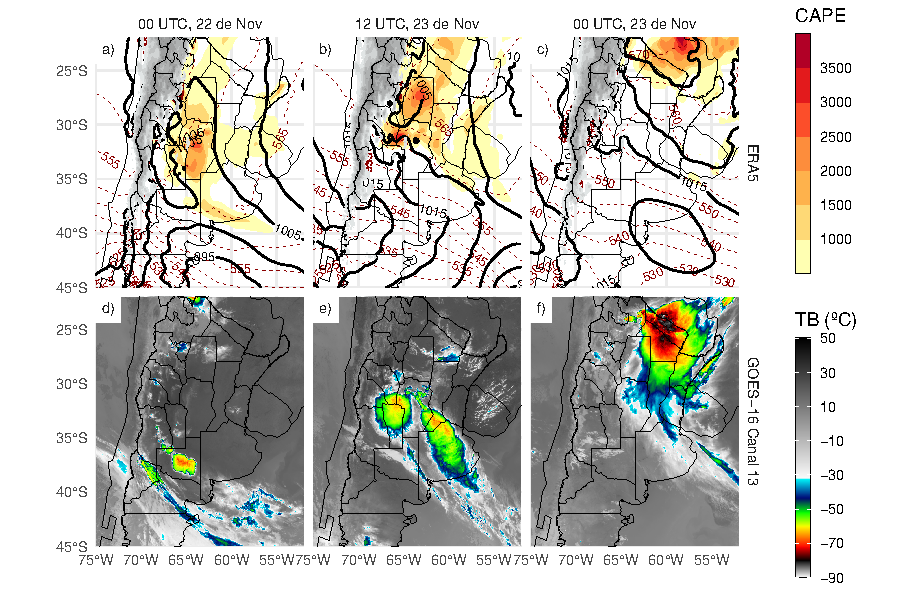
\includegraphics{thesis_files/figure-latex/caso-1} 

}

\caption{Presión a nivel del mar (hPa, contornos negros), espesor 1000-500 hPa (contornos rojos discontinuos) y energía potencial convectiva disponible (sombreada) según ERA5 y temperatura de brillo del canal 13 de GOES-16 para a,d) 00 y b,e) 12 UTC, 22 de Nov y c,f) 00 UTC, 23 de Nov.~}\label{fig:caso}
\end{figure}
\hypertarget{configuraciuxf3n-del-ensamble}{%
\section{Configuración del ensamble}\label{configuraciuxf3n-del-ensamble}}

Las simulaciones numéricas para el caso de estudio se realizan utilizando la versión 3.9.1 de modelo WRF (Skamarock et al. (2008)).
Se utilizó una resolución horizontal de 10 km (150 x 200 puntos de retícula) y 37 niveles en la vertical con el tope del modelo en 50 hPa.
Las condiciones iniciales y de contorno surgen del análisis del Global Forecast System (GFS) (resolución horizontal de 0,25\(^{\circ}\) y resolución temporal de 6 horas; National Centers for Environmental Prediction, National Weather Service, NOAA, U.S. Department of Commerce (2015)).
El dominio cubre la zona indicada en la Figura \ref{fig:dominio} para capturar el desarrollo del SCM durante el periodo simulado.

Los análisis se generaron utilizando la implementación LETKF (V1.3, Hunt et al. (2007)) que forma parte del sistema de análisis Gridpoint Statistical Interpolation (GSI V3.8; Shao et al. (2016)).
Se utilizó un enfoque de actualización rápida con análisis horario y una ventana de asimilación centrada, lo que significa que se asimilaron todas las observaciones dentro de \(\pm\) 30 minutos del tiempo de análisis.
Además, aas observaciones se asimilaron usando un enfoque 4D, es decir, comparándolas con el first guess más cercano que se genera en intervalos de 10 minutos.
Para las observaciones de satelite, se utilizó el Community Radiative Transfer Model versión 2.3 (CRTM; Han et al. (2006)) como operador de observaciones para calcular las temperaturas de brillo simuladas por el modelo.

Utilizamos un conjunto de 60 miembros, cuya media al principio del ciclo de AD se inicializa utilizando el análisis deterministico del GFS al que se le suman perturbaciones aleatorias para generar el ensamble incial. Las perturbaciones se generaron como diferencias escaladas entre dos estados atmosféricos aleatorios obtenidos a partir de los datos del Reanálisis del Sistema de Predicción del Clima (CFSR) con una resolución horizontal de 0,5\(^{\circ}\) que tiene una con una evolución temporal suave (Necker et al., 2020; Maldonado et al., 2021). De este modo, preservamos el equilibrio casi hidrostático y geostrófico de las escalas mayores. Este método ayuda a evitar una subestimación del spread del ensamble (Ouaraini et al., 2015). Las perturbaciones también se aplicaron en los límites para mantener niveles adecuados de spread dentro del dominio del ensamble.

Además de las perturbaciones aleatorias en los límites laterales, se utilizó un esquema de multifísicas para representar mejor la incertidumbre en el modelo dentro del sistema de AD. Utilizamos 9 configuraciones diferentes que consisten en la combinación de 3 esquemas de convección húmeda (Kain-Fritsch (Kain, 2004), Grell-Freitas (Grell and Freitas, 2013), y Betts-Miller-Janjic (Janjić, 1994)) y 3 esquemas de capa límite planetaria (Esquema de la Universidad de Yonsei (Hong, Noh, et al., 2006), Esquema Mellor-Yamada-Janjic (Janjić, 1994), y Mellor-Yamada Nakanishi Niino (Nakanishi and Niino, 2009)). La distribución de estas parametrizaciones entre los 60 miembros del ensamble se muestra en la Tabla \ref{tab:miembros-desc}. Todos los miembros del conjunto utilizan las mismas parametrizaciones del modelo de superficie terrestre (Noah-MP, Chen and Dudhia (2001)), de microfísica (esquema de un solo momento de 6 clases del WRF (Hong, Kim, et al., 2006)) y de procesos radiativos (esquema de onda corta y onda larga del RRTMG (Iacono et al., 2008)).
\begin{table}

\caption{\label{tab:miembros-desc}Generación de los 60 miembros del ensamble multifísica como combinación de parametrizaciones de Cumulus y PBL}
\centering
\fontsize{9}{11}\selectfont
\begin{tabular}[t]{c>{\centering\arraybackslash}p{8em}>{\centering\arraybackslash}p{8em}>{\centering\arraybackslash}p{8em}}
\toprule
\multicolumn{1}{c}{ } & \multicolumn{3}{c}{PBL} \\
\cmidrule(l{3pt}r{3pt}){2-4}
Cumulus & MYJ & MYNN2 & YSU\\
\midrule
BMJ & 5, 14, 23, 32, 41, 50, 59 & 8, 17, 26, 35, 44, 53 & 2, 11, 20, 29, 38, 47, 56\\
GF & 6, 15, 24, 33, 42, 51, 60 & 9, 18, 27, 36, 45, 54 & 3, 12, 21, 30, 39, 48, 57\\
KF & 4, 13, 22, 31, 40, 49, 58 & 7, 16, 25, 34, 43, 52 & 1, 10, 19, 28, 37, 46, 55\\
\bottomrule
\end{tabular}
\end{table}
Para reducir el efecto de las correlaciones espurias en la estimación de las covarianzas de los errores de las observaciones, utilizamos un radio de localización horizontal de 180 km y un radio de localización vertical de 0,4 (en coordenadas de presión logarítmica) como en Dillon et al. (2021) para todos los tipos de observaciones.
Se aplicó con un parámetro de inflación \(\alpha=0,9\) para mitigar el impacto de los errores de muestreo y para considerar los errores del modelo que no se tienen en cuenta en el enfoque mutifísica del ensamble (Whitaker and Hamill, 2012).


\begin{figure}

{\centering 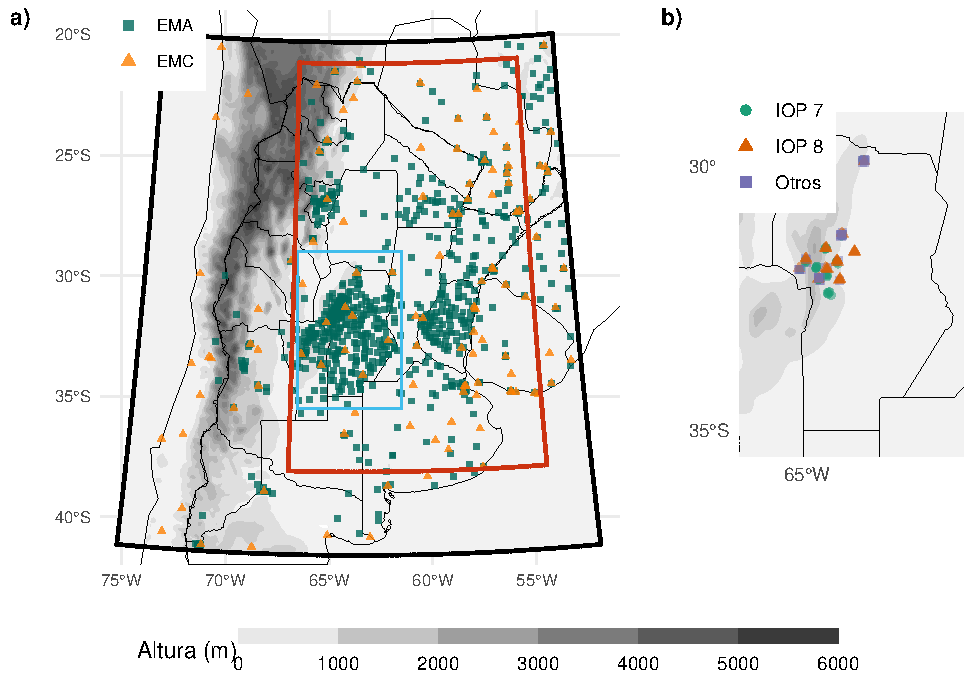
\includegraphics[width=0.8\linewidth]{thesis_files/figure-latex/dominio-1} 

}

\caption{a) Dominio utilizado para las simulaciones (recuadro negro), dominio interior utilizado para la comparación entre experimentos (recuadro rojo), la región mostrada en b) (recuadro azul claro), y la ubicación de las Estaciones Meteorológicas Automáticas (EMA, cuadrados verdes) y las Estaciones Meteorológicas Convencionales (EMC, triángulos naranjas). b) Ubicación de los lanzamientos de radiosondeos durante RELAMPAGO. Los puntos verdes corresponden a los radiosondeos lanzados durante el IOP 7, los triángulos naranjas son radiosondeos lanzados durante el IOP 8, y los cuadrados morados son radiosondeos lanzados fuera de los periodos de medición intensiva. También se muestra la topografía en metros (sombreada).}\label{fig:dominio}
\end{figure}
\hypertarget{verificaciuxf3n-obs-y-metricas}{%
\section{Verificación: obs y metricas}\label{verificaciuxf3n-obs-y-metricas}}

\hypertarget{conjunto-de-datos-de-validaciuxf3n}{%
\subsection{Conjunto de datos de validación}\label{conjunto-de-datos-de-validaciuxf3n}}

Para evaluar el desempeño del sistema AD presentado en esta tesis, utilizamos los siguientes conjuntos de observaciones:
\begin{itemize}
\item
  \textbf{Datos horarios en niveles de presión de ERA5 de 1959 al presente (Hersbach et al., 2018):} Las variables de interés (temperatura del aire, humedad y viento) fueron interpoladas a la retícula del modelo para compararlas con el análisis de cada experimento.
\item
  \textbf{Multi-Network Composite Highest Resolution Radiosonde Data (Earth Observing Laboratory, 2020):} radiosondeos en alta resolución lanzados desde varias ubicaciones durante el periodo de la campaña de campo de RELAMPAGO en junto con las radiosondeos operativos del SMN. Sólo se utilizaron para la validación los sondeos que no ingresaron en el sistema de asimilación. El periodo del experimento abarca las misiones IOP 7 y 8, durante las cuales se lanzaron 74 radiosondos en una pequeña zona cercana al centro del dominio experimental (Figura \ref{fig:dominio}b).
\item
  \textbf{IMERG Final Run (Huffman et al., 2018):} estimación de la precipitación a partir de datos de la constelación de satelites GPM (por su nombre en inglés Global Precipitation Measurement) con una resolución espacial de 0,01\(^{circ}\) y una resolución temporal de 30 minutos para validar la habilidad de los pronósticos de 1 hora para representar la precipitación sobre el dominio.
\item
  \textbf{Datos del Sistema Nacional de Radares Meteorológicos (SINARAME):} Se utilizaron observaciones de radar para realizar una evaluación cualitativa y visual de las características convectivas. Los datos provienen de 9 radares ubicados en el dominio y son provistos por la red de radares Doppler de doble polarización en banda C (de Elía et al., 2017) con una frecuencia temporal de 10 minutos. Para este trabajo se utilizó únicamente la máxima reflectividad de la columna (COLMAX) más cercana al momento de análisis.
\end{itemize}
\hypertarget{muxe9todos-de-verificaciuxf3n}{%
\subsection{Métodos de verificación}\label{muxe9todos-de-verificaciuxf3n}}

Se seleccionaron un conjunto de métricas para evaluar diferentes aspectos del análisis obtenido para cada experimento y los pronósticos inicializados a partir de ellos. Estas métricas incluyen una validación de cómo se cuantifica la incertidumbre en el first guess y en el análisis, y cómo los diferentes experimentos se ajustan a un conjunto independiente de observaciones que no se asimilan.

Para evaluar la consistencia de la estimación de la incertidumbre en el first guess y en el análisis utilizamos la Reduced Centered Random Variable o RCRV (Candille et al. (2007)) que se define como:
\begin{equation}
  \mathrm{RCRV = \frac{m - x_o}{\sqrt{\sigma_o^2 + \sigma^2}}}
  \label{eq:eq6}
\end{equation}
donde \(x_o\) es la observación asimilada y su error \(\sigma_o\), \(m\) la media ensamble del análisis en el espacio de las observaciones, y la desviación estándar \(\sigma\) del ensamble
La media de \(RCRV\) calculada sobre todas las realizaciones representa el sesgo de la media del conjunto con respecto a las observaciones normalizadas por la incertidumbre estimada:
\begin{equation}
  \mathrm{\mathit{mean RCRV} = E[RCRV]}
  \label{eq:eq7}
\end{equation}
La desviación estándar de la \(RCRV\) o \(sd RCRV\) mide la concordancia de la dispersión del ensamble y el error de observación con respecto a la distancia entre la media del ensamble y las observaciones, y por lo tanto, la sobre o infradispersión sistemática del ensamble:
\begin{equation}
  \mathrm{\mathit{sd RCRV} = \sqrt{\frac{1}{M -1}\sum_{i=1}^{M}(\mathit{RCRV_i} - \mathit{mean RCRV})^2}}
  \label{eq:eq8}
\end{equation}
donde \(M\) es el tamaño del ensamble. Suponiendo que el error de observación fue estimado con precisión, un \(sd RCRV > 1\) indica que el ensamble es infradispersivo (es decir, la distancia entre las observaciones y los pronósticos es mayor de lo esperado), y un \(sd RCRV < 1\) indica que el conjunto es sobredispersivo (es decir, la distancia entre las observaciones y los pronósticos es menor de lo esperado). Un sistema consistente no tendrá sesgo (\(media RCRV = 0\)) y una desviación estándar igual a 1 (\(sd RCRV = 1\)).

Para analizar el ajuste del first guess y el análisis a un conjunto de observaciones independientes, los radiosondeos de alta resolución de RELAMPAGO, se calculó la raiz del error cuadrático medio (RMSE) y el BIAS:
\begin{equation}
  \mathrm{\mathit{RMSE} = \sqrt{\frac{1}{N}\sum_{i = 1}^{N} (X_i - O_i)^{2}}}
  \label{eq:eq9}
\end{equation}
\begin{equation}
  \mathrm{\mathit{BIAS} = \frac{1}{N}\sum_{i = 1}^{N} (X_i - O_i)}
  \label{eq:eq10}
\end{equation}
donde \(O\) y \(X\) representan las observaciones independientes y las simuladas respectivamente, y N es el tamaño de la muestra.

Para comparar la pricipitación pronísticada a 1 hora con las estimaciones de precipitación de IMERG, calculamos el Fractions Skill Score (FSS, Roberts (2008)) para diferentes radios de influencia y umbrales de precipitación:
\begin{equation}
  \mathrm{\mathit{FSS} = 1-\frac{\sum_{i=1}^{N} ({P_x}_i-{P_o}_i)^{2}}{\sum_{i=1}^{N} ({P_x}_i)^{2}+\sum_{i=1}^{N} ({P_o}_i)^{2}}}
    \label{eq:eq11}
\end{equation}
donde \(P_{oi}\) es la proporción de puntos de reticula en el subdominio \(i-th\) donde la que la precipitación acumulada observada es mayor que un umbral especificado. Siguiendo a Roberts et al. (2020), \(P_{xi}\) se calcula sobre el ensamble completo y cuantifica de la probabilidad de que la precipitación sea mayor al mismo umbral en cada punto de cuadrícula, y luego promediando sobre el subdominio \(i-th\).
El FSS se calculó a partir de la precipitación acumulada en ventanas moviles de 6 horas sumando los pronósticos de precipitación acumulada de 1 hora.

\hypertarget{recursos-computacionales}{%
\section{Recursos computacionales}\label{recursos-computacionales}}

Todos los experimentos corrieron en la supercomputadora Cheyenne del Centro Nacional de Investigación Atmosférica (NCAR) (Computational and Information Systems Laboratory, 2019). El posprocesamineto y análisis se realizó en {[}CIMA{]}. El análisis de datos se generó utilizando el lenguaje de programación R (R Core Team, 2020), utilizando los paquetes data.table (Dowle and Srinivasan, 2020) y metR (Campitelli, 2020), entre otros.
Todos los gráficos se han realizado con ggplot2 (Wickham, 2009) y la versión final de la tesis se generó con knitr, rmarkdown (Xie, 2015; Allaire et al., 2019) y tesisdown {[}{]}.

\hypertarget{asimilacion-de-observaciones-de-estaciones-meteoroluxf3gicas-automuxe1ticas-vientos-derivados-de-satuxe9lite-y-radianzas-de-satelites-polares}{%
\chapter{Asimilacion de observaciones de estaciones meteorológicas automáticas, vientos derivados de satélite y radianzas de satelites polares}\label{asimilacion-de-observaciones-de-estaciones-meteoroluxf3gicas-automuxe1ticas-vientos-derivados-de-satuxe9lite-y-radianzas-de-satelites-polares}}

\hypertarget{presentaciuxf3n-y-metodologuxeda}{%
\section{Presentación y metodología}\label{presentaciuxf3n-y-metodologuxeda}}

\hypertarget{observaciones-asimiladas}{%
\subsection{Observaciones asimiladas}\label{observaciones-asimiladas}}

\hypertarget{conventional}{%
\subsubsection{Conventional}\label{conventional}}

The conventional observations used are part of the Global Data Assimilation System (GDAS) data stream. Conventional observations included in the Binary Universal Form for Representation of Meteorological Data (PREPBUFR) files generated at the National Centers for Environmental Prediction (NCEP) are assimilated. These consist of surface observations from 117 Conventional Surface Weather Stations (CSWS), ships, and upper-air observations from 13 radiosondes sites and aircraft. The orange triangles in Figure \ref{fig:dominio}a indicate the location of the surface stations included in this experiment. The frequency of these observations varied between 1 hour for surface stations and 12/24 hours for radiosondes. Wind surface observations over oceans (ASCATW) come from scatterometers and are also included in the PREPBUFR files.

Table \ref{tab:table-obs} lists all the observation types (i.e., surface pressure, temperature, specific humidity, and wind) available for each source, together with their associated errors. The observation errors were specified following the GSI default configuration. In some cases, the error varies with height and depends on the specific platform (aircraft and satellite-derived wind). In terms of quality control, a gross check was performed by the observation operator by comparing the innovation (the difference between the observation and the model-simulated observation based on the first-guess) with a predefined threshold that depends on the observation error (also included in Table \ref{tab:table-obs}).

\hypertarget{aws-networks}{%
\subsubsection{AWS networks}\label{aws-networks}}

Data from 866 Automatic Weather Stations (AWS) that are part of 17 public and private surface networks over Southern South America are also assimilated. The dataset used in this study has been obtained from the RELAMPAGO Data Set repository (Garcia et al., 2019). These stations are indicated as green squares in Figure \ref{fig:dominio}a. They have higher spatial coverage than the CSWS and a sampling frequency of 10 minutes in most cases. All stations measure temperature, but only 395 stations provide humidity, 422 provide pressure, and 605 provide wind information.
Observation errors used to assimilate these observations are the same as for the CSWS (see Table \ref{tab:table-obs}).

\hypertarget{satellite-derived-winds}{%
\subsubsection{Satellite-derived winds}\label{satellite-derived-winds}}

Satellite-derived wind observations are also included in the PREPBUFR files available every 6 h, and consist of estimations from GOES-16 (using the visible, infrared, and water vapor channels) and METEOSAT 8 and 11 (using the visible and water vapor channels). Due to the domain covered by each of these satellites, GOES-16 is the primary source of satellite-derived winds (99 \% of the observations). Observation errors used to assimilate these observations follow the GSI default configuration and are indicated in Table \ref{tab:table-obs}.
\begin{table}

\caption{\label{tab:table-obs}Characteristics of the assimilated observations: The code for each observation type and its source, the available variables, the observation error, and the gross check thresholds used.}
\centering
\fontsize{9}{11}\selectfont
\begin{tabular}[t]{>{\raggedright\arraybackslash}p{4.5em}>{\raggedright\arraybackslash}p{5.5em}>{\raggedright\arraybackslash}p{6em}>{\raggedright\arraybackslash}p{8em}>{\raggedright\arraybackslash}p{8em}}
\toprule
Code & Platform & Variable & Error & Gross check\\
\midrule
 &  & Pressure & 1-1.6 $hPa^*$ & 3.6 $hPa$\\

 &  & Temperature & 1.5 $K$ & 7 $K$\\

 &  & Specific humidity & 20 \% & 8 $gKg^{-1}$\\

\multirow{-4}{4.5em}{\raggedright\arraybackslash CSWS   AWS} & \multirow{-4}{5.5em}{\raggedright\arraybackslash Surface weather stations} & Wind & 2.2 $ms^{-1}$ & 6 $ms^{-1}$\\
\cmidrule{1-5}
 &  & Pressure & 1.1-1.2 $hPa^{**}$ & 4 $hPa$\\

 &  & Temperature & 0.8-1.5 $K^*$ & 8 $K$\\

 &  & Specific humidity & 20 \% & 8 $gKg^{-1}$\\

\multirow{-4}{4.5em}{\raggedright\arraybackslash ADPUPA} & \multirow{-4}{5.5em}{\raggedright\arraybackslash Radiosondes} & Wind & 1.4-3 $ms^{-1}$* & 8 $ms^{-1}$\\
\cmidrule{1-5}
 &  & Temperature & 1.47-2.5 $K^+$ & 7 $K$\\

\multirow{-2}{4.5em}{\raggedright\arraybackslash AIRCFT} & \multirow{-2}{5.5em}{\raggedright\arraybackslash Aircrafts} & Wind & 2.4-3.6 $ms^{-1+}$ & 6.5-7.5 $ms^{-1+}$\\
\cmidrule{1-5}
ASCATW & Advanced Scatterometers & Wind & 1.5 $ms^{-1}$ & 5 $ms^{-1}$\\
\cmidrule{1-5}
 &  & Pressure & 1.3 $hPa$ & 4 $hPa$\\

 &  & Temperature & 2.5 $K$ & 7 $K$\\

 &  & Specific humidity & 20 \% & 8 $gKg^{-1}$\\

\multirow{-4}{4.5em}{\raggedright\arraybackslash SFCSHP} & \multirow{-4}{5.5em}{\raggedright\arraybackslash Ships and Buoys} & Wind & 2.5 $ms^{-1}$ & 5 $ms^{-1}$\\
\cmidrule{1-5}
SATWND & Satellite-derived winds & Wind & 3.8-8 $ms^{-1*+}$ & 1.3-2.5 $ms^{-1+}$\\
\bottomrule
\multicolumn{5}{l}{\rule{0pt}{1em}\textsuperscript{*} Observation error varied with height.}\\
\multicolumn{5}{l}{\rule{0pt}{1em}\textsuperscript{**} Observations above 600 hPa are rejected.}\\
\multicolumn{5}{l}{\rule{0pt}{1em}\textsuperscript{+} Observation error depends on the report type.}\\
\end{tabular}
\end{table}
\hypertarget{sat}{%
\subsubsection{Satellite radiances}\label{sat}}

Satellite radiances available through the GDAS data stream, consisting of infrared and microwave observations, are used in this study. This includes the Advanced Microwave Sounding Unit - A (AMSU-A), Microwave Humidity Sounder (MHS), and 2 multispectral sensors; the Atmospheric Infrared Sounder (AIRS) and the Infrared Atmospheric Sounding Interferometer (IASI) over several satellite platforms (see Table \ref{tab:table-rad}). Since the regional domain is located in the mid-latitudes and the satellite platforms of interest are on polar orbits, each sensor scans the area only twice a day with a spatial coverage depending on the satellite swath. For this reason, the number of satellite observations varied significantly among cycles. In particular, the multispectral sensors provided between 100 and 1000 observations for every scan every 12 hours, contributing 88 \% of the total amount of assimilated radiances in our experiment. The vertical location of each radiance observation was estimated as the model level at which its weighting function was maximized as calculated by CRTM. The multispectral sensors have good vertical coverage and are able to sense from the lower troposphere up to the lower stratosphere.

The channels adopted for assimilation and their associated errors were defined taking into account the low model top (50 hPa). The data preprocessing, which is an essential step in the assimilation of radiances, was performed within the GSI system for each sensor specifically. First, a spatial data thinning is applied using a 60 km grid following Singh et al. (2016), Jones et al. (2013), and Lin et al. (2017), where the observations to be assimilated are chosen based on their distance to the model grid points, the observation quality (based on available data quality information), and the number of available channels (from the same pixel and sensor) that passed the quality control. Also, observations over the sea are preferred to those over land or snow (Hu et al., 2018).

The thinned observations were then bias corrected. The bias correction (BC) has an air-mass dependent and an angle-dependent component (Zhu et al., 2014) and it is calculated as a multi-linear function of N predictors \(p_i(x)\), with associated coefficients \(\beta_i\). Then, the bias corrected brightness temperature (\(BT_{bc}\)) can be obtained as:
\begin{equation}
  \mathrm{\mathit{BT_{bc}} =\mathit{ BT} + \sum_{i = 0}^{N} \beta_i p_i (x)}
  \label{eq:eq12}
\end{equation}
GSI has a constant offset bias correction term (\(p_0 = 1\)) and the remaining predictors are the cloud liquid water content (CLW), the temperature lapse rate at the pressure of maximum weight, the square of the temperature lapse rate at the pressure of maximum weight, and the emissivity sensitivity. Scan angle-dependent bias is modeled as a 4th-order polynomial (Zhu et al., 2014).

In the GSI system, the \(\beta_i\) coefficients are trained using a variational estimation method which solves the \(\beta_i\) that provides the best fit between the simulation and the observations. The coefficients were initialized at 18 UTC Nov 18, 2018 with the GFS system coefficients. The assimilation system was configured to use a constant background error variance of 0.01 to avoid large adjustments in the estimated coefficients at each time.

In our experiments, only clear-sky observations are used. For microwave radiances, observations potentially contaminated by clouds are detected using the scattering and Liquid Water Path (LWP) indexes (Zhu et al., 2016; Weston et al., 2019). For the infrared channels, cloud contaminated observations are detected using the transmittance profile calculated within the CRTM algorithms. Moreover, GSI checks the difference between the observations and simulated brightness temperature with height to detect cloudy pixels. Additionally, the GSI quality control for infrared sensors looks for observations over water with a large zenith angle (over 60°) to reject channels near the visible range that can be contaminated with reflection. It also performs an emissivity check for observations over land for both infrared and microwave radiances.
\begin{table}

\caption{\label{tab:table-rad}List of the available sensors over several platforms, the number of accepted channels for the assimilation, and the percentage of assimilated observations calculated over all radiance observations and all cycles.}
\centering
\fontsize{9}{11}\selectfont
\begin{tabu} to \linewidth {>{\raggedright}X>{\raggedright}X>{\raggedleft}X>{\raggedright}X}
\toprule
Sensor & Platform & Assimilated channels & Percentage over total\\
\midrule
AIRS & AQUA & 52 & 31.63 \%\\
\cmidrule{1-4}
 & NOAA15 & 2 & 3.31 \%\\
\cmidrule{2-4}
 & NOAA18 & 2 & 4.45 \%\\
\cmidrule{2-4}
\multirow[t]{-3}{*}{\raggedright\arraybackslash AMSUA} & METOP-A & 2 & 2.08 \%\\
\cmidrule{1-4}
 & METOP-A & 66 & 52.72 \%\\
\cmidrule{2-4}
\multirow[t]{-2}{*}{\raggedright\arraybackslash IASI} & METOP-B & 68 & 3.47 \%\\
\cmidrule{1-4}
 & NOAA19 & 2 & 0.68 \%\\
\cmidrule{2-4}
 & METOP-A & 3 & 0.8 \%\\
\cmidrule{2-4}
\multirow[t]{-3}{*}{\raggedright\arraybackslash MHS} & METOP-B & 3 & 0.85 \%\\
\bottomrule
\end{tabu}
\end{table}

\begin{figure}
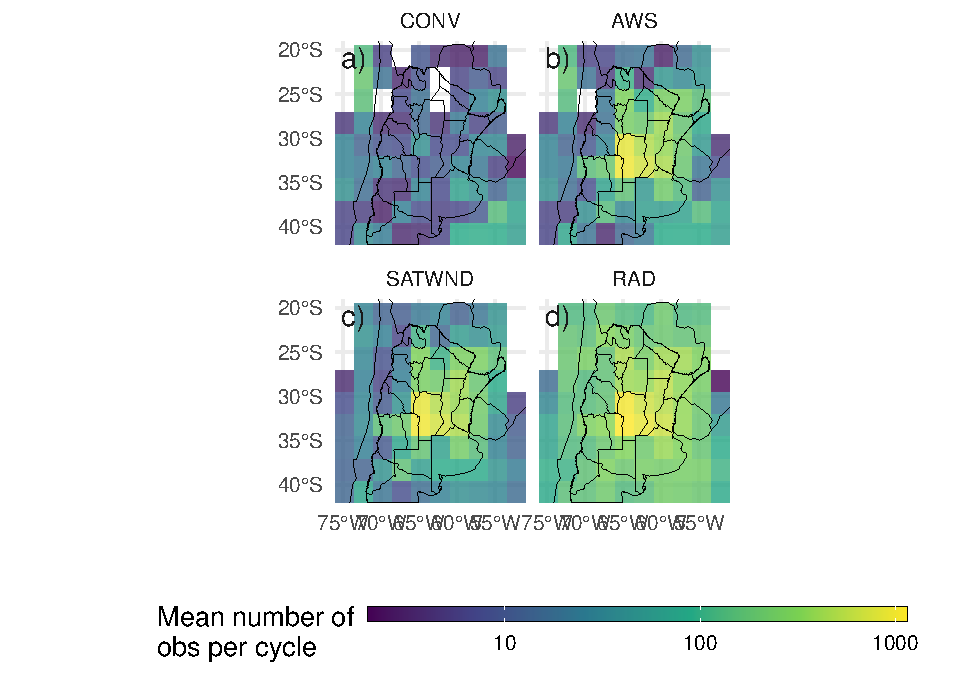
\includegraphics[width=1\linewidth]{thesis_files/figure-latex/obs-horizontal-1} \caption{Horizontal spatial distribution of the mean available observations per analysis cycle for the a) CONV, b) AWS, c) SATWND, and d) RAD experiments calculated over 2.5\(^{\circ}\) boxes.}\label{fig:obs-horizontal}
\end{figure}

\begin{figure}
\centering
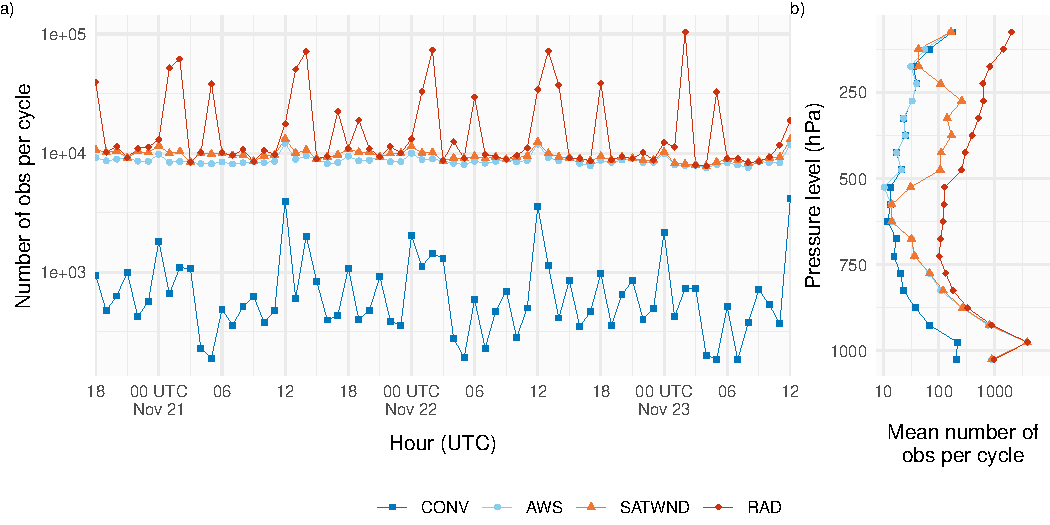
\includegraphics{thesis_files/figure-latex/obs-cycle-1.pdf}
\caption{\label{fig:obs-cycle}a) Number of assimilated observations per cycle and b) time averaged number of assimilated observations per cycle divided into 50 hPa-depth vertical layers for the CONV (blue squares and line), AWS (light blue dots and line), SATWND (orange triangles and line) and RAD (red diamonds and line) experiments.}
\end{figure}
\hypertarget{configuracion-de-los-experimentos}{%
\subsection{Configuracion de los experimentos}\label{configuracion-de-los-experimentos}}

To investigate the impact of different observations upon the analysis, four DA experiments were performed using different observation sets (Table \ref{tab:table-exp}). The CONV experiment uses only conventional observations from PREPBUFR. In a second experiment, referred to as AWS, all the observations included in CONV are assimilated plus the 10-minute frequency surface observations from AWS. In the third experiment, referred to as SATWND, the observations from the AWS experiment along with the satellite-derived winds are assimilated. Finally, a fourth experiment referred to as RAD assimilates all available clear-sky radiances from sensors onboard polar orbiting satellites as described in section \ref{sat}.
\begin{table}

\caption{\label{tab:table-exp}Observation types assimilated in each experiment.}
\centering
\begin{tabu} to \linewidth {>{\raggedright\arraybackslash}p{8em}>{\centering\arraybackslash}m{2.5em}>{\centering\arraybackslash}m{2.5em}>{\centering\arraybackslash}m{3em}>{\centering\arraybackslash}m{3em}}
\toprule
Obs type & CONV & AWS & SATWND & RAD\\
\midrule
Conventional (PREPBUFR) & x & x & x & x\\
Conventional (AWS) &  & x & x & x\\
Satellite-derived winds &  &  & x & x\\
Radiances &  &  &  & x\\
\bottomrule
\end{tabu}
\end{table}
The horizontal distribution of the average number of assimilated observations per cycle in each experiment is shown in Figure \ref{fig:obs-horizontal}. The larger number of assimilated observations over the center and east of the domain corresponds to the AWS observations. In Figure \ref{fig:obs-cycle}a the number of assimilated observations over time is shown. Local maxima at 12 and 00 UTC found mainly in CONV are attributed to operational soundings. The strong variability in the number of radiance observations per cycle is also noticeable and depends on the satellite coverage. The maxima at 13-14 and 01-02 UTC in RAD correspond to the contribution of the multispectral sensors. The vertical distribution of the mean number of observations per cycle (Figure \ref{fig:obs-cycle}b) shows a maximum in low levels due to the AWS observations. Satellite-derived winds are maximized at the upper troposphere (between 500-250 hPa). Above 850 hPa, most of the observations correspond to radiance observations.

All the assimilation experiments start at 18 UTC Nov 20, 2018 and continue until 12 UTC Nov, 23 (totaling 67 hours/assimilation cycles). The initial 60-member ensemble is generated as explained in section \ref{config} from a spin-up run without assimilating observations performed between 12 UTC and 18 UTC Nov, 20 (Figure \ref{fig:cycle}).


\begin{figure}
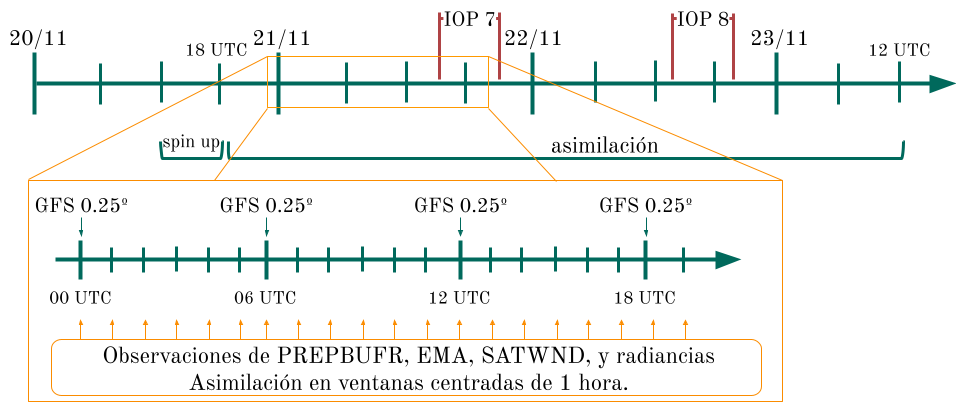
\includegraphics[width=0.8\linewidth]{/home/paola.corrales/tesis_doctorado/figure/analysis_cycle} \caption{Diagram of the analysis cycles between 18 UTC Nov 20, and 12 UTC Nov 23 plus spin up period of 6 hours. The zoomed section shows the hourly assimilation that is performed within a one-hour centered window and new boundary conditions from GFS every 6 hours. The two IOP missions from the RELAMPAGO field campaign and the ensemble forecast initialized at 00 and 06 UTC Nov 22 are shown.}\label{fig:cycle}
\end{figure}
\hypertarget{resultados}{%
\section{Resultados}\label{resultados}}

\hypertarget{ensamble}{%
\subsection{Ensamble}\label{ensamble}}

\hypertarget{impacto-en-el-analisis}{%
\subsection{Impacto en el analisis}\label{impacto-en-el-analisis}}

\hypertarget{verificacion}{%
\subsection{Verificacion}\label{verificacion}}

\hypertarget{conclusiones}{%
\subsection{Conclusiones}\label{conclusiones}}

\hypertarget{ref-labels}{%
\chapter{Graphics, References, and Labels}\label{ref-labels}}

\hypertarget{figures}{%
\section{Figures}\label{figures}}

If your thesis has a lot of figures, \emph{R Markdown} might behave better for you than that other word processor. One perk is that it will automatically number the figures accordingly in each chapter. You'll also be able to create a label for each figure, add a caption, and then reference the figure in a way similar to what we saw with tables earlier. If you label your figures, you can move the figures around and \emph{R Markdown} will automatically adjust the numbering for you. No need for you to remember! So that you don't have to get too far into LaTeX to do this, a couple \textbf{R} functions have been created for you to assist. You'll see their use below.

In the \textbf{R} chunk below, we will load in a picture stored as \texttt{reed.jpg} in our main directory. We then give it the caption of ``Reed logo'', the label of ``reedlogo'', and specify that this is a figure. Make note of the different \textbf{R} chunk options that are given in the R Markdown file (not shown in the knitted document).
\begin{figure}

{\centering 
\includegraphics[width=0.2\linewidth]{figure/reed} 

}

\caption{Reed logo}\label{fig:reedlogo}
\end{figure}
Here is a reference to the Reed logo: Figure \ref{fig:reedlogo}. Note the use of the \texttt{fig:} code here. By naming the \textbf{R} chunk that contains the figure, we can then reference that figure later as done in the first sentence here. We can also specify the caption for the figure via the R chunk option \texttt{fig.cap}.

\clearpage

Below we will investigate how to save the output of an \textbf{R} plot and label it in a way similar to that done above. Recall the \texttt{flights} dataset from Chapter \ref{rmd-basics}. (Note that we've shown a different way to reference a section or chapter here.) We will next explore a bar graph with the mean flight departure delays by airline from Portland for 2014.
\begin{figure}
\centering
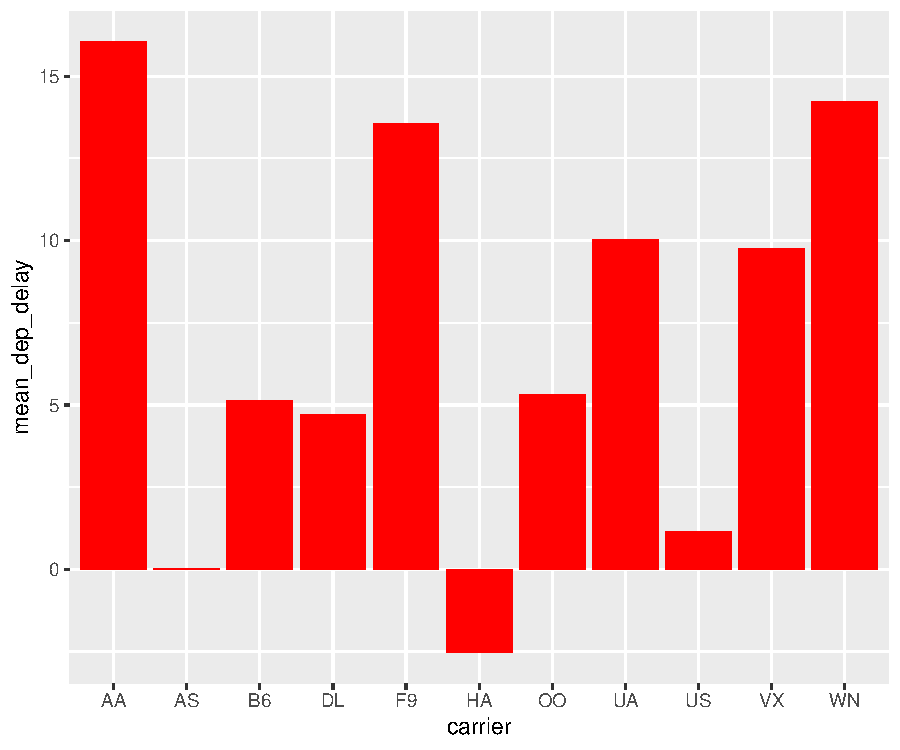
\includegraphics{thesis_files/figure-latex/delaysboxplot-1.pdf}
\caption{\label{fig:delaysboxplot}Mean Delays by Airline}
\end{figure}
Here is a reference to this image: Figure \ref{fig:delaysboxplot}.

A table linking these carrier codes to airline names is available at \url{https://github.com/ismayc/pnwflights14/blob/master/data/airlines.csv}.

\clearpage

Next, we will explore the use of the \texttt{out.extra} chunk option, which can be used to shrink or expand an image loaded from a file by specifying \texttt{"scale=\ "}. Here we use the mathematical graph stored in the ``subdivision.pdf'' file.
\begin{figure}
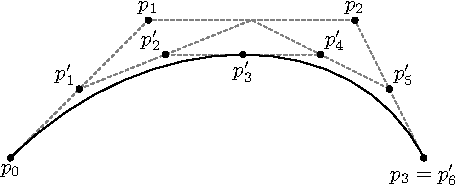
\includegraphics[scale=0.75]{figure/subdivision} \caption{Subdiv. graph}\label{fig:subd}
\end{figure}
Here is a reference to this image: Figure \ref{fig:subd}. Note that \texttt{echo=FALSE} is specified so that the \textbf{R} code is hidden in the document.

\textbf{More Figure Stuff}

Lastly, we will explore how to rotate and enlarge figures using the \texttt{out.extra} chunk option. (Currently this only works in the PDF version of the book.)
\begin{figure}
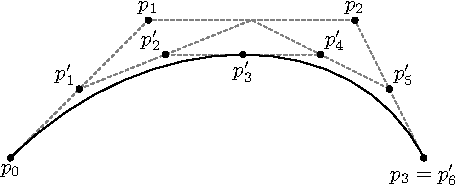
\includegraphics[angle=180, scale=1.1]{figure/subdivision} \caption{A Larger Figure, Flipped Upside Down}\label{fig:subd2}
\end{figure}
As another example, here is a reference: Figure \ref{fig:subd2}.

\hypertarget{footnotes-and-endnotes}{%
\section{Footnotes and Endnotes}\label{footnotes-and-endnotes}}

You might want to footnote something.\footnote{footnote text} The footnote will be in a smaller font and placed appropriately. Endnotes work in much the same way. More information can be found about both on the CUS site or feel free to reach out to \href{mailto:data@reed.edu}{\nolinkurl{data@reed.edu}}.

\hypertarget{bibliographies}{%
\section{Bibliographies}\label{bibliographies}}

Of course you will need to cite things, and you will probably accumulate an armful of sources. There are a variety of tools available for creating a bibliography database (stored with the .bib extension). In addition to BibTeX suggested below, you may want to consider using the free and easy-to-use tool called Zotero. The Reed librarians have created Zotero documentation at \url{https://libguides.reed.edu/citation/zotero}. In addition, a tutorial is available from Middlebury College at \url{https://sites.middlebury.edu/zoteromiddlebury/}.

\emph{R Markdown} uses \emph{pandoc} (\url{https://pandoc.org/}) to build its bibliographies. One nice caveat of this is that you won't have to do a second compile to load in references as standard LaTeX requires. To cite references in your thesis (after creating your bibliography database), place the reference name inside square brackets and precede it by the ``at'' symbol. For example, here's a reference to a book about worrying: ({\textbf{???}}). This \texttt{Molina1994} entry appears in a file called \texttt{thesis.bib} in the \texttt{bib} folder. This bibliography database file was created by a program called BibTeX. You can call this file something else if you like (look at the YAML header in the main .Rmd file) and, by default, is to placed in the \texttt{bib} folder.

For more information about BibTeX and bibliographies, see our CUS site (\url{https://web.reed.edu/cis/help/latex/index.html})\footnote{({\textbf{???}})}. There are three pages on this topic: \emph{bibtex} (which talks about using BibTeX, at \url{https://web.reed.edu/cis/help/latex/bibtex.html}), \emph{bibtexstyles} (about how to find and use the bibliography style that best suits your needs, at \url{https://web.reed.edu/cis/help/latex/bibtexstyles.html}) and \emph{bibman} (which covers how to make and maintain a bibliography by hand, without BibTeX, at \url{https://web.reed.edu/cis/help/latex/bibman.html}). The last page will not be useful unless you have only a few sources.

If you look at the YAML header at the top of the main .Rmd file you can see that we can specify the style of the bibliography by referencing the appropriate csl file. You can download a variety of different style files at \url{https://www.zotero.org/styles}. Make sure to download the file into the csl folder.

\vfill

\textbf{Tips for Bibliographies}
\begin{itemize}
\tightlist
\item
  Like with thesis formatting, the sooner you start compiling your bibliography for something as large as thesis, the better. Typing in source after source is mind-numbing enough; do you really want to do it for hours on end in late April? Think of it as procrastination.
\item
  The cite key (a citation's label) needs to be unique from the other entries.
\item
  When you have more than one author or editor, you need to separate each author's name by the word ``and'' e.g.~\texttt{Author\ =\ \{Noble,\ Sam\ and\ Youngberg,\ Jessica\},}.
\item
  Bibliographies made using BibTeX (whether manually or using a manager) accept LaTeX markup, so you can italicize and add symbols as necessary.
\item
  To force capitalization in an article title or where all lowercase is generally used, bracket the capital letter in curly braces.
\item
  You can add a Reed Thesis citation\footnote{({\textbf{???}})} option. The best way to do this is to use the phdthesis type of citation, and use the optional ``type'' field to enter ``Reed thesis'' or ``Undergraduate thesis.''
\end{itemize}
\hypertarget{anything-else}{%
\section{Anything else?}\label{anything-else}}

If you'd like to see examples of other things in this template, please contact the Data @ Reed team (email \href{mailto:data@reed.edu}{\nolinkurl{data@reed.edu}}) with your suggestions. We love to see people using \emph{R Markdown} for their theses, and are happy to help.

\hypertarget{conclusion}{%
\chapter*{Conclusion}\label{conclusion}}
\addcontentsline{toc}{chapter}{Conclusion}

If we don't want Conclusion to have a chapter number next to it, we can add the \texttt{\{-\}} attribute.

\textbf{More info}

And here's some other random info: the first paragraph after a chapter title or section head \emph{shouldn't be} indented, because indents are to tell the reader that you're starting a new paragraph. Since that's obvious after a chapter or section title, proper typesetting doesn't add an indent there.

\appendix

\hypertarget{the-first-appendix}{%
\chapter{The First Appendix}\label{the-first-appendix}}

This first appendix includes all of the R chunks of code that were hidden throughout the document (using the \texttt{include\ =\ FALSE} chunk tag) to help with readibility and/or setup.

\textbf{In the main Rmd file}
\begin{Shaded}
\begin{Highlighting}[]
\CommentTok{# This chunk ensures that the thesisdown package is}
\CommentTok{# installed and loaded. This thesisdown package includes}
\CommentTok{# the template files for the thesis.}
\ControlFlowTok{if}\NormalTok{ (}\OperatorTok{!}\KeywordTok{require}\NormalTok{(remotes)) \{}
  \ControlFlowTok{if}\NormalTok{ (params}\OperatorTok{$}\StringTok{`}\DataTypeTok{Install needed packages for \{thesisdown\}}\StringTok{`}\NormalTok{) \{}
    \KeywordTok{install.packages}\NormalTok{(}\StringTok{"remotes"}\NormalTok{, }\DataTypeTok{repos =} \StringTok{"https://cran.rstudio.com"}\NormalTok{)}
\NormalTok{  \} }\ControlFlowTok{else}\NormalTok{ \{}
    \KeywordTok{stop}\NormalTok{(}
      \KeywordTok{paste}\NormalTok{(}\StringTok{'You need to run install.packages("remotes")",}
\StringTok{            "first in the Console.'}\NormalTok{)}
\NormalTok{    )}
\NormalTok{  \}}
\NormalTok{\}}
\ControlFlowTok{if}\NormalTok{ (}\OperatorTok{!}\KeywordTok{require}\NormalTok{(thesisdown)) \{}
  \ControlFlowTok{if}\NormalTok{ (params}\OperatorTok{$}\StringTok{`}\DataTypeTok{Install needed packages for \{thesisdown\}}\StringTok{`}\NormalTok{) \{}
\NormalTok{    remotes}\OperatorTok{::}\KeywordTok{install_github}\NormalTok{(}\StringTok{"ismayc/thesisdown"}\NormalTok{)}
\NormalTok{  \} }\ControlFlowTok{else}\NormalTok{ \{}
    \KeywordTok{stop}\NormalTok{(}
      \KeywordTok{paste}\NormalTok{(}
        \StringTok{"You need to run"}\NormalTok{,}
        \StringTok{'remotes::install_github("ismayc/thesisdown")'}\NormalTok{,}
        \StringTok{"first in the Console."}
\NormalTok{      )}
\NormalTok{    )}
\NormalTok{  \}}
\NormalTok{\}}
\KeywordTok{library}\NormalTok{(thesisdown)}
\CommentTok{# Set how wide the R output will go}
\KeywordTok{options}\NormalTok{(}\DataTypeTok{width =} \DecValTok{70}\NormalTok{)}
\end{Highlighting}
\end{Shaded}
\textbf{In Chapter \ref{ref-labels}:}
\begin{Shaded}
\begin{Highlighting}[]
\CommentTok{# This chunk ensures that the thesisdown package is}
\CommentTok{# installed and loaded. This thesisdown package includes}
\CommentTok{# the template files for the thesis and also two functions}
\CommentTok{# used for labeling and referencing}
\ControlFlowTok{if}\NormalTok{ (}\OperatorTok{!}\KeywordTok{require}\NormalTok{(remotes)) \{}
  \ControlFlowTok{if}\NormalTok{ (params}\OperatorTok{$}\StringTok{`}\DataTypeTok{Install needed packages for \{thesisdown\}}\StringTok{`}\NormalTok{) \{}
    \KeywordTok{install.packages}\NormalTok{(}\StringTok{"remotes"}\NormalTok{, }\DataTypeTok{repos =} \StringTok{"https://cran.rstudio.com"}\NormalTok{)}
\NormalTok{  \} }\ControlFlowTok{else}\NormalTok{ \{}
    \KeywordTok{stop}\NormalTok{(}
      \KeywordTok{paste}\NormalTok{(}
        \StringTok{'You need to run install.packages("remotes")'}\NormalTok{,}
        \StringTok{"first in the Console."}
\NormalTok{      )}
\NormalTok{    )}
\NormalTok{  \}}
\NormalTok{\}}
\ControlFlowTok{if}\NormalTok{ (}\OperatorTok{!}\KeywordTok{require}\NormalTok{(dplyr)) \{}
  \ControlFlowTok{if}\NormalTok{ (params}\OperatorTok{$}\StringTok{`}\DataTypeTok{Install needed packages for \{thesisdown\}}\StringTok{`}\NormalTok{) \{}
    \KeywordTok{install.packages}\NormalTok{(}\StringTok{"dplyr"}\NormalTok{, }\DataTypeTok{repos =} \StringTok{"https://cran.rstudio.com"}\NormalTok{)}
\NormalTok{  \} }\ControlFlowTok{else}\NormalTok{ \{}
    \KeywordTok{stop}\NormalTok{(}
      \KeywordTok{paste}\NormalTok{(}
        \StringTok{'You need to run install.packages("dplyr")'}\NormalTok{,}
        \StringTok{"first in the Console."}
\NormalTok{      )}
\NormalTok{    )}
\NormalTok{  \}}
\NormalTok{\}}
\ControlFlowTok{if}\NormalTok{ (}\OperatorTok{!}\KeywordTok{require}\NormalTok{(ggplot2)) \{}
  \ControlFlowTok{if}\NormalTok{ (params}\OperatorTok{$}\StringTok{`}\DataTypeTok{Install needed packages for \{thesisdown\}}\StringTok{`}\NormalTok{) \{}
    \KeywordTok{install.packages}\NormalTok{(}\StringTok{"ggplot2"}\NormalTok{, }\DataTypeTok{repos =} \StringTok{"https://cran.rstudio.com"}\NormalTok{)}
\NormalTok{  \} }\ControlFlowTok{else}\NormalTok{ \{}
    \KeywordTok{stop}\NormalTok{(}
      \KeywordTok{paste}\NormalTok{(}
        \StringTok{'You need to run install.packages("ggplot2")'}\NormalTok{,}
        \StringTok{"first in the Console."}
\NormalTok{      )}
\NormalTok{    )}
\NormalTok{  \}}
\NormalTok{\}}
\ControlFlowTok{if}\NormalTok{ (}\OperatorTok{!}\KeywordTok{require}\NormalTok{(bookdown)) \{}
  \ControlFlowTok{if}\NormalTok{ (params}\OperatorTok{$}\StringTok{`}\DataTypeTok{Install needed packages for \{thesisdown\}}\StringTok{`}\NormalTok{) \{}
    \KeywordTok{install.packages}\NormalTok{(}\StringTok{"bookdown"}\NormalTok{, }\DataTypeTok{repos =} \StringTok{"https://cran.rstudio.com"}\NormalTok{)}
\NormalTok{  \} }\ControlFlowTok{else}\NormalTok{ \{}
    \KeywordTok{stop}\NormalTok{(}
      \KeywordTok{paste}\NormalTok{(}
        \StringTok{'You need to run install.packages("bookdown")'}\NormalTok{,}
        \StringTok{"first in the Console."}
\NormalTok{      )}
\NormalTok{    )}
\NormalTok{  \}}
\NormalTok{\}}
\ControlFlowTok{if}\NormalTok{ (}\OperatorTok{!}\KeywordTok{require}\NormalTok{(thesisdown)) \{}
  \ControlFlowTok{if}\NormalTok{ (params}\OperatorTok{$}\StringTok{`}\DataTypeTok{Install needed packages for \{thesisdown\}}\StringTok{`}\NormalTok{) \{}
\NormalTok{    remotes}\OperatorTok{::}\KeywordTok{install_github}\NormalTok{(}\StringTok{"ismayc/thesisdown"}\NormalTok{)}
\NormalTok{  \} }\ControlFlowTok{else}\NormalTok{ \{}
    \KeywordTok{stop}\NormalTok{(}
      \KeywordTok{paste}\NormalTok{(}
        \StringTok{"You need to run"}\NormalTok{,}
        \StringTok{'remotes::install_github("ismayc/thesisdown")'}\NormalTok{,}
        \StringTok{"first in the Console."}
\NormalTok{      )}
\NormalTok{    )}
\NormalTok{  \}}
\NormalTok{\}}
\KeywordTok{library}\NormalTok{(thesisdown)}
\KeywordTok{library}\NormalTok{(dplyr)}
\KeywordTok{library}\NormalTok{(ggplot2)}
\KeywordTok{library}\NormalTok{(knitr)}
\NormalTok{flights <-}\StringTok{ }\KeywordTok{read.csv}\NormalTok{(}\StringTok{"data/flights.csv"}\NormalTok{, }\DataTypeTok{stringsAsFactors =} \OtherTok{FALSE}\NormalTok{)}
\end{Highlighting}
\end{Shaded}
\hypertarget{the-second-appendix-for-fun}{%
\chapter{The Second Appendix, for Fun}\label{the-second-appendix-for-fun}}

\backmatter

\hypertarget{references}{%
\chapter*{References}\label{references}}
\addcontentsline{toc}{chapter}{References}

\markboth{References}{References}

\noindent

\setlength{\parindent}{-0.20in}

\hypertarget{refs}{}
\leavevmode\hypertarget{ref-aksoy2010}{}%
Aksoy, A., Dowell, D.C., and Snyder, C., 2010. A Multicase Comparative Assessment of the Ensemble Kalman Filter for Assimilation of Radar Observations. Part II: Short-Range Ensemble Forecasts. Monthly Weather Review, 138, 4, 1273--1292.

\leavevmode\hypertarget{ref-allaire2019}{}%
Allaire, J., Horner, J., Xie, Y., Marti, V., and Porte, N., 2019. Markdown: Render markdown with the c library 'sundown'.

\leavevmode\hypertarget{ref-andersson1991}{}%
Andersson, E., Hollingsworth, A., Kelly, G., Lönnberg, P., Pailleux, J., and Zhang, Z., 1991. Global Observing System Experiments on Operational Statistical Retrievals of Satellite Sounding Data. Monthly Weather Review, 119, 8, 1851--1865.

\leavevmode\hypertarget{ref-bae2022}{}%
Bae, J.-H., and Min, K.-H., 2022. Forecast Characteristics of Radar Data Assimilation Based on the Scales of Precipitation Systems. Remote Sensing, 14, 3, 3, 605.

\leavevmode\hypertarget{ref-bao2015}{}%
Bao, Y., Xu, J., Powell Jr., A.M., Shao, M., Min, J., and Pan, Y., 2015. Impacts of AMSU-A, MHS and IASI data assimilation on temperature and humidity forecasts with GSI--WRF over the western United States. Atmospheric Measurement Techniques, 8, 10, 4231--4242.

\leavevmode\hypertarget{ref-baucemachado2017}{}%
Bauce Machado, V., gustavo de goncalves, luis, Vendrasco, E., Sinhori, N., Herdies, D., Sapucci, L., Levien, C., Quadro, M., Rodrigues, T., and Cardoso, C. and others, 2017. Investigating the impacts of convective scale hazardous weather events in Santa Catarina State through the CPTEC/INPE local data assimilation system. In. Presented at the Seventh International WMO Symposium on Data Assimilation.

\leavevmode\hypertarget{ref-campitelli2020}{}%
Campitelli, E., 2020, April. metR: Tools for Easier Analysis of Meteorological Fields.

\leavevmode\hypertarget{ref-candille2007}{}%
Candille, G., Côté, C., Houtekamer, P.L., and Pellerin, G., 2007. Verification of an Ensemble Prediction System against Observations. Monthly Weather Review, 135, 7, 2688--2699.

\leavevmode\hypertarget{ref-chang2017}{}%
Chang, W., Jacques, D., Fillion, L., and Baek, S.-J., 2017. Assimilation of Hourly Surface Observations with the Canadian High-Resolution Ensemble Kalman Filter. Atmosphere-Ocean, 55, 4-5, 247--263.

\leavevmode\hypertarget{ref-chen2001}{}%
Chen, F., and Dudhia, J., 2001. Coupling an Advanced Land Surface--Hydrology Model with the Penn State--NCAR MM5 Modeling System. Part I: Model Implementation and Sensitivity. Monthly Weather Review, 129, 4, 569--585.

\leavevmode\hypertarget{ref-chen2016}{}%
Chen, X., Zhao, K., Sun, J., Zhou, B., and Lee, W.-C., 2016. Assimilating surface observations in a four-dimensional variational Doppler radar data assimilation system to improve the analysis and forecast of a squall line case. Advances in Atmospheric Sciences, 33, 10, 1106--1119.

\leavevmode\hypertarget{ref-cherubini2006}{}%
Cherubini, T., Businger, S., Velden, C., and Ogasawara, R., 2006. The Impact of Satellite-Derived Atmospheric Motion Vectors on Mesoscale Forecasts over Hawaii. Monthly Weather Review, 134, 7, 2009--2020.

\leavevmode\hypertarget{ref-clark2009}{}%
Clark, A.J., Gallus, W.A., Xue, M., and Kong, F., 2009. A Comparison of Precipitation Forecast Skill between Small Convection-Allowing and Large Convection-Parameterizing Ensembles. Weather and Forecasting, 24, 4, 1121--1140.

\leavevmode\hypertarget{ref-Cheyenne2019}{}%
Computational and Information Systems Laboratory, 2019. Cheyenne: HPE/SGI ICE XA System (University Community Computing). National Center for Atmospheric Research Boulder, CO.

\leavevmode\hypertarget{ref-deelia2017}{}%
de Elía, R., Vidal, L., and Lohigorry, P., 2017. El SMN y la red argentina de radares meteorológicos (\url{http://hdl.handle.net/20.500.12160/625}).

\leavevmode\hypertarget{ref-dillon2021}{}%
Dillon, M.E., Maldonado, P., Corrales, P., Skabar, Y.G., Ruiz, J., Sacco, M., Cutraro, F., Mingari, L., Matsudo, C., and Vidal, L. and others, 2021. A rapid refresh ensemble based data assimilation and forecast system for the RELAMPAGO field campaign. Atmospheric Research, 105858.

\leavevmode\hypertarget{ref-dowle2020}{}%
Dowle, M., and Srinivasan, A., 2020, July. Data.Table: Extension of 'data.frame'.

\leavevmode\hypertarget{ref-sondeos}{}%
Earth Observing Laboratory, U. -, 2020. Multi-network composite highest resolution radiosonde data. Version 1.3. UCAR/NCAR - earth observing laboratory.

\leavevmode\hypertarget{ref-eyre2020}{}%
Eyre, J.R., English, S.J., and Forsythe, M., 2020. Assimilation of satellite data in numerical weather prediction. Part I: The early years. Quarterly Journal of the Royal Meteorological Society, 146, 726, 49--68.

\leavevmode\hypertarget{ref-eyre2022}{}%
Eyre, J.R., Bell, W., Cotton, J., English, S.J., Forsythe, M., Healy, S.B., and Pavelin, E.G., 2022. Assimilation of satellite data in numerical weather prediction. Part II: Recent years. Quarterly Journal of the Royal Meteorological Society, 148, 743, 521--556.

\leavevmode\hypertarget{ref-ferreira2017}{}%
Ferreira, R.C., Herdies, D.L., Vendrasco, É.P., Beneti, C.A.A., and Biscaro, T.S., 2017. Impacto da Assimilação de Dados de Radar em Sistemas Convectivos de Mesoescala: Um Estudo de Caso. Revista Brasileira de Meteorologia, 32, 3, 447--458.

\leavevmode\hypertarget{ref-ferreira2020}{}%
Ferreira, R.C., Alves Júnior, M.P., Vendrasco, éder P., Aravéquia, J.A., Nolasco Junior, L.R., Biscaro, T.S., Ferreira, R.C., Alves Júnior, M.P., Vendrasco, éder P., and Aravéquia, J.A. and others, 2020. The Impact of Microphysics Parameterization on Precipitation Forecast Using Radar Data Assimilation. Revista Brasileira de Meteorologia, 35, 1, 123--134.

\leavevmode\hypertarget{ref-gao2015}{}%
Gao, F., Huang, X.-Y., Jacobs, N.A., and Wang, H., 2015. Assimilation of wind speed and direction observations: Results from real observation experiments. Tellus A: Dynamic Meteorology and Oceanography, 67, 1, 27132.

\leavevmode\hypertarget{ref-garcia2019}{}%
Garcia, F., Ruiz, J., Salio, P., Bechis, H., and Nesbitt, S., 2019. Argentina mesonet data. Version 1.1. UCAR/NCAR - earth observing laboratory.

\leavevmode\hypertarget{ref-garciaskabar1997}{}%
García Skabar, Y., 1997. Análisis objetivo regional para inicializar un modelo de diez niveles en forma operativa. Tesis de licenciatura en ciencias de la atmósfera.

\leavevmode\hypertarget{ref-gasperoni2018}{}%
Gasperoni, N.A., Wang, X., Brewster, K.A., and Carr, F.H., 2018. Assessing Impacts of the High-Frequency Assimilation of Surface Observations for the Forecast of Convection Initiation on 3 April 2014 within the Dallas--Fort Worth Test Bed. Monthly Weather Review, 146, 11, 3845--3872.

\leavevmode\hypertarget{ref-goncalvesdegoncalves2015}{}%
Goncalves de Goncalves, L.G., Sapucci, L., Vendrasco, E., de Mattos, J.G., Ferreira, C., Khamis, E., and Cruz, N., 2015. A rapid update data assimilation cycle over South America using 3DVar and EnKF. In The 20th International TOVS Study Conference (ITSC-20).

\leavevmode\hypertarget{ref-grell2013}{}%
Grell, G.A., and Freitas, S.R., 2013. A scale and aerosol aware stochastic convective parameterization for weather and air quality modeling. Atmospheric Chemistry and Physics Discussions, 13, 9, 23845--23893.

\leavevmode\hypertarget{ref-ha2014}{}%
Ha, S.-Y., and Snyder, C., 2014. Influence of Surface Observations in Mesoscale Data Assimilation Using an Ensemble Kalman Filter. Monthly Weather Review, 142, 4, 1489--1508.

\leavevmode\hypertarget{ref-han2006}{}%
Han, Y., Van Delst, P., Liu, Q., Weng, F., Yan, B., Treadon, R., and Derber, J., 2006. JCSDA Community Radiative Transfer Model (CRTM)---version 1 p. 40.

\leavevmode\hypertarget{ref-era5pressure}{}%
Hersbach, H., Bell, B., Berrisford, P., Biavati, G., Horányi, A., Muñoz Sabater, J., Nicolas, J., Peubey, C., Radu, R., and Rozum, I. and others, 2018. ERA5 hourly data on pressure levels from 1959 to present. Copernicus Climate Change Service (C3S) Climate Data Store (CDS), (Accessed on \(<\)08-08-2022\(>\)).

\leavevmode\hypertarget{ref-hong2006}{}%
Hong, S.-Y., Noh, Y., and Dudhia, J., 2006. A New Vertical Diffusion Package with an Explicit Treatment of Entrainment Processes. Monthly Weather Review, 134, 9, 2318--2341.

\leavevmode\hypertarget{ref-hong2006a}{}%
Hong, S.-Y., Kim, J.-H., Lim, J.-o., and Dudhia, J., 2006. The WRF Single Moment 6-Class Microphysics Scheme (WSM6). Journal of the Korean Meteorological Society, 42, 129--151.

\leavevmode\hypertarget{ref-hu2018}{}%
Hu, M., Ge, G., Zhou, C., Stark, D., Shao, H., Newman, K., Beck, J., and Zhang, X., 2018. Grid-point Statistical Interpolation (GSI) User's Guide Version 3.7, Developmental Testbed Center, p. 149.

\leavevmode\hypertarget{ref-huffman2018}{}%
Huffman, G., Bolvin, D., Braithwaite, D., Hsu, K., Joyce, R., Kidd, C., Nelkin, E., Sorooshian, S., Tan, J., and Xie, P., 2018. NASA Global Precipitation Measurement (GPM) Integrated Multi-satellitE Retrievals for GPM (IMERG), National Aeronautics and Space Administration (NASA), p. 35.

\leavevmode\hypertarget{ref-hunt2007}{}%
Hunt, B.R., Kostelich, E.J., and Szunyogh, I., 2007. Efficient data assimilation for spatiotemporal chaos: A local ensemble transform Kalman filter. Physica D: Nonlinear Phenomena, 230, 1-2, 112--126.

\leavevmode\hypertarget{ref-iacono2008}{}%
Iacono, M.J., Delamere, J.S., Mlawer, E.J., Shephard, M.W., Clough, S.A., and Collins, W.D., 2008. Radiative forcing by long-lived greenhouse gases: Calculations with the AER radiative transfer models. Journal of Geophysical Research, 113, D13, D13103.

\leavevmode\hypertarget{ref-janjic1994}{}%
Janjić, Z.I., 1994. The Step-Mountain Eta Coordinate Model: Further Developments of the Convection, Viscous Sublayer, and Turbulence Closure Schemes. Monthly Weather Review, 122, 5, 927--945.

\leavevmode\hypertarget{ref-jones2013}{}%
Jones, T.A., Otkin, J.A., Stensrud, D.J., and Knopfmeier, K., 2013. Assimilation of Satellite Infrared Radiances and Doppler Radar Observations during a Cool Season Observing System Simulation Experiment. Monthly Weather Review, 141, 10, 3273--3299.

\leavevmode\hypertarget{ref-kain2004}{}%
Kain, J.S., 2004. The Kain--Fritsch Convective Parameterization: An Update. JOURNAL OF APPLIED METEOROLOGY, 43, 12.

\leavevmode\hypertarget{ref-kalnay2002}{}%
Kalnay, E., 2002, November 6. Atmospheric Modeling, Data Assimilation and Predictability (\url{https://www.cambridge.org/highereducation/books/atmospheric-modeling-data-assimilation-and-predictability/C5FD207439132836E85027754CE9BC1A}).

\leavevmode\hypertarget{ref-kelly1978}{}%
Kelly, G.a.M., Mills, G.A., and Smith, W.L., 1978. Impact of Nimbus-6 Temperature Soundings on Australian Region Forecasts. Bulletin of the American Meteorological Society, 59, 4, 393--406.

\leavevmode\hypertarget{ref-kleist2009}{}%
Kleist, D.T., Parrish, D.F., Derber, J.C., Treadon, R., Wu, W.-S., and Lord, S., 2009. Introduction of the GSI into the NCEP Global Data Assimilation System. Weather and Forecasting, 24, 6, 1691--1705.

\leavevmode\hypertarget{ref-lin2017a}{}%
Lin, H., Weygandt, S.S., Benjamin, S.G., and Hu, M., 2017. Satellite Radiance Data Assimilation within the Hourly Updated Rapid Refresh. Weather and Forecasting, 32, 4, 1273--1287.

\leavevmode\hypertarget{ref-maejima2019}{}%
Maejima, Y., Miyoshi, T., Kunii, M., Seko, H., and Sato, K., 2019. Impact of Dense and Frequent Surface Observations on 1-Minute-Update Severe Rainstorm Prediction: A Simulation Study. Journal of the Meteorological Society of Japan. Ser. II, 97, 1, 253--273.

\leavevmode\hypertarget{ref-maldonado2021}{}%
Maldonado, P., Ruiz, J., and Saulo, C., 2021. Sensitivity to Initial and Boundary Perturbations in Convective-Scale Ensemble-Based Data Assimilation: Imperfect-Model OSSEs. SOLA, 17, 0, 96--102.

\leavevmode\hypertarget{ref-nakanishi2009}{}%
Nakanishi, M., and Niino, H., 2009. Development of an Improved Turbulence Closure Model for the Atmospheric Boundary Layer. Journal of the Meteorological Society of Japan, 87, 5, 895--912.

\leavevmode\hypertarget{ref-cisl_rda_ds084.1}{}%
National Centers for Environmental Prediction, National Weather Service, NOAA, U.S. Department of Commerce, 2015. NCEP GFS 0.25 degree global forecast grids historical archive.

\leavevmode\hypertarget{ref-necker2020}{}%
Necker, T., Geiss, S., Weissmann, M., Ruiz, J., Miyoshi, T., and Lien, G., 2020. A convective‐scale 1,000‐member ensemble simulation and potential applications. Quarterly Journal of the Royal Meteorological Society, 146, 728, 1423--1442.

\leavevmode\hypertarget{ref-nesbitt2021}{}%
Nesbitt, S.W., Salio, P.V., Ávila, E., Bitzer, P., Carey, L., Chandrasekar, V., Deierling, W., Dominguez, F., Dillon, M.E., and Garcia, C.M. and others, 2021. A storm safari in Subtropical South America: Proyecto RELAMPAGO. Bulletin of the American Meteorological Society, -1, aop, 1--64.

\leavevmode\hypertarget{ref-ohring1979}{}%
Ohring, G., 1979. Impact of Satellite Temperature Sounding Data on Weather Forecasts. Bulletin of the American Meteorological Society, 60, 10, 1142--1147.

\leavevmode\hypertarget{ref-ouaraini2015}{}%
Ouaraini, R.E., Berre, L., Fischer, C., and Sayouty, E.H., 2015. Sensitivity of regional ensemble data assimilation spread to perturbations of lateral boundary conditions. Tellus A: Dynamic Meteorology and Oceanography, 67, 1, 28502.

\leavevmode\hypertarget{ref-pondeca2011}{}%
Pondeca, M.S.F.V.D., Manikin, G.S., DiMego, G., Benjamin, S.G., Parrish, D.F., Purser, R.J., Wu, W.-S., Horel, J.D., Myrick, D.T., and Lin, Y. and others, 2011. The Real-Time Mesoscale Analysis at NOAA's National Centers for Environmental Prediction: Current Status and Development. Weather and Forecasting, 26, 5, 593--612.

\leavevmode\hypertarget{ref-purser2003a}{}%
Purser, R.J., Wu, W.-S., Parrish, D.F., and Roberts, N.M., 2003a. Numerical Aspects of the Application of Recursive Filters to Variational Statistical Analysis. Part II: Spatially Inhomogeneous and Anisotropic General Covariances. Monthly Weather Review, 131, 8, 1536--1548.

\leavevmode\hypertarget{ref-purser2003}{}%
---------, 2003b. Numerical Aspects of the Application of Recursive Filters to Variational Statistical Analysis. Part I: Spatially Homogeneous and Isotropic Gaussian Covariances. Monthly Weather Review, 131, 8, 1524--1535.

\leavevmode\hypertarget{ref-rcoreteam2020}{}%
R Core Team, 2020. R: A language and environment for statistical computing, R Foundation for Statistical Computing,

\leavevmode\hypertarget{ref-roberts2020}{}%
Roberts, B., Gallo, B.T., Jirak, I.L., Clark, A.J., Dowell, D.C., Wang, X., and Wang, Y., 2020. What Does a Convection-Allowing Ensemble of Opportunity Buy Us in Forecasting Thunderstorms? Weather and Forecasting, 35, 6, 2293--2316.

\leavevmode\hypertarget{ref-roberts2008}{}%
Roberts, N., 2008. Assessing the spatial and temporal variation in the skill of precipitation forecasts from an NWP model. Meteorological Applications, 15, 1, 163--169.

\leavevmode\hypertarget{ref-saucedo}{}%
Saucedo, M.A., n.d. Estudio de los efectos de diferentes fuentes de error sobre la calidad de los análisis generados por un sistema de asimilación por filtros de Kalman, 279.

\leavevmode\hypertarget{ref-sawada2019}{}%
Sawada, M., Ma, Z., Mehra, A., Tallapragada, V., Oyama, R., and Shimoji, K., 2019. Impacts of Assimilating High-Resolution Atmospheric Motion Vectors Derived from Himawari-8 on Tropical Cyclone Forecast in HWRF. Monthly Weather Review, 147, 10, 3721--3740.

\leavevmode\hypertarget{ref-shao2016}{}%
Shao, H., Derber, J., Huang, X.-Y., Hu, M., Newman, K., Stark, D., Lueken, M., Zhou, C., Nance, L., and Kuo, Y.-H. and others, 2016. Bridging Research to Operations Transitions: Status and Plans of Community GSI. Bulletin of the American Meteorological Society, 97, 8, 1427--1440.

\leavevmode\hypertarget{ref-singh2016}{}%
Singh, R., Ojha, S.P., Kishtawal, C.M., Pal, P.K., and Kiran Kumar, A.S., 2016. Impact of the assimilation of INSAT-3D radiances on short-range weather forecasts: Assimilation of INSAT-3D Radiances. Quarterly Journal of the Royal Meteorological Society, 142, 694, 120--131.

\leavevmode\hypertarget{ref-skamarock2008}{}%
Skamarock, W.C., Klemp, J.B., Dudhia, J., Gill, D.O., Barker, D.M., Duda, M.G., Huang, X.-Y., Wang, W., and Powers, J.G., 2008. A Description of the Advanced Research WRF Version 3 p. 125.

\leavevmode\hypertarget{ref-sobash2015}{}%
Sobash, R.A., and Stensrud, D.J., 2015. Assimilating Surface Mesonet Observations with the EnKF to Improve Ensemble Forecasts of Convection Initiation on 29 May 2012. Monthly Weather Review, 143, 9, 3700--3725.

\leavevmode\hypertarget{ref-stensrud2013}{}%
Stensrud, D.J., Wicker, L.J., Xue, M., Dawson, D.T., Yussouf, N., Wheatley, D.M., Thompson, T.E., Snook, N.A., Smith, T.M., and Schenkman, A.D. and others, 2013. Progress and challenges with Warn-on-Forecast. Atmospheric Research, 123, 2--16.

\leavevmode\hypertarget{ref-toshioinouye2017}{}%
Toshio Inouye, R., Calvetti, L., Gonçalves, J., Maske, B., Neundorf, R., Beneti, C., Diniz, F., Vendrasco, E., Herdies, D., and gustavo de goncalves, luis, 2017. Impact of radar data assimilation on a severe storm study in brazil. In. Presented at the 97th American Meteorological Meeting Annual Meeting.

\leavevmode\hypertarget{ref-vera1992}{}%
Vera, C.S., 1992. Un sistema de asimilación de datos para la región extratropical de Sudamérica.

\leavevmode\hypertarget{ref-wang2021}{}%
Wang, Z.Q., and Randriamampianina, R., 2021. The Impact of Assimilating Satellite Radiance Observations in the Copernicus European Regional Reanalysis (CERRA). Remote Sensing, 13, 3, 3, 426.

\leavevmode\hypertarget{ref-weston2019}{}%
Weston, P., Geer, A., Bormann, N., and Bormann, N., 2019. Investigations into the assimilation of AMSU-A in the presence of cloud and precipitation.

\leavevmode\hypertarget{ref-wheatley2010}{}%
Wheatley, D.M., and Stensrud, D.J., 2010. The Impact of Assimilating Surface Pressure Observations on Severe Weather Events in a WRF Mesoscale Ensemble System. Monthly Weather Review, 138, 5, 1673--1694.

\leavevmode\hypertarget{ref-whitaker2002}{}%
Whitaker, J.S., and Hamill, T.M., 2002. Ensemble Data Assimilation without Perturbed Observations. Monthly Weather Review, 130, 7, 1913--1924.

\leavevmode\hypertarget{ref-whitaker2012}{}%
---------, 2012. Evaluating Methods to Account for System Errors in Ensemble Data Assimilation. Monthly Weather Review, 140, 9, 3078--3089.

\leavevmode\hypertarget{ref-whitaker2008}{}%
Whitaker, J.S., Hamill, T.M., Wei, X., Song, Y., and Toth, Z., 2008. Ensemble Data Assimilation with the NCEP Global Forecast System. Monthly Weather Review, 136, 2, 463--482.

\leavevmode\hypertarget{ref-wickham2009}{}%
Wickham, H., 2009. Ggplot2: Elegant Graphics for Data Analysis, Springer-Verlag,

\leavevmode\hypertarget{ref-wu2014}{}%
Wu, T.-C., Liu, H., Majumdar, S.J., Velden, C.S., and Anderson, J.L., 2014. Influence of Assimilating Satellite-Derived Atmospheric Motion Vector Observations on Numerical Analyses and Forecasts of Tropical Cyclone Track and Intensity. Monthly Weather Review, 142, 1, 49--71.

\leavevmode\hypertarget{ref-wu2002}{}%
Wu, W.-S., Purser, R.J., and Parrish, D.F., 2002. Three-Dimensional Variational Analysis with Spatially Inhomogeneous Covariances. Monthly Weather Review, 130, 12, 2905--2916.

\leavevmode\hypertarget{ref-xie2015}{}%
Xie, Y., 2015. Dynamic documents with R and knitr, Second., Chapman and Hall/CRC,

\leavevmode\hypertarget{ref-zhu2019}{}%
Zhu, K., Xue, M., Pan, Y., Hu, M., Benjamin, S.G., Weygandt, S.S., and Lin, H., 2019. The Impact of Satellite Radiance Data Assimilation within a Frequently Updated Regional Forecast System Using a GSI-based Ensemble Kalman Filter. Advances in Atmospheric Sciences, 36, 12, 1308--1326.

\leavevmode\hypertarget{ref-zhu2008}{}%
Zhu, Y., and Gelaro, R., 2008. Observation Sensitivity Calculations Using the Adjoint of the Gridpoint Statistical Interpolation (GSI) Analysis System. Monthly Weather Review, 136, 1, 335--351.

\leavevmode\hypertarget{ref-zhu2014}{}%
Zhu, Y., Derber, J., Collard, A., Dee, D., Treadon, R., Gayno, G., and Jung, J.A., 2014. Enhanced radiance bias correction in the National Centers for Environmental Prediction's Gridpoint Statistical Interpolation data assimilation system. Quarterly Journal of the Royal Meteorological Society, 140, 682, 1479--1492.

\leavevmode\hypertarget{ref-zhu2016}{}%
Zhu, Y., Liu, E., Mahajan, R., Thomas, C., Groff, D., Van Delst, P., Collard, A., Kleist, D., Treadon, R., and Derber, J.C., 2016. All-Sky Microwave Radiance Assimilation in NCEP's GSI Analysis System. Monthly Weather Review, 144, 12, 4709--4735.


% Index?

\end{document}
